\documentclass{etutez}
\usepackage{graphicx}
\usepackage[toc,page,titletoc]{appendix}
\usepackage[T1]{fontenc}
\usepackage[utf8]{inputenc}
\usepackage[turkish]{babel}
\usepackage{titlesec}
\usepackage{longtable}
\usepackage{mathtools}



\pagenumbering{roman}

\thesistype{M.Sc.} %Yuksek lisans icin M.Sc. doktora icin Ph.D.
\teztipi{Yüksek Lisans}  %Tez tipini yazin

\keywords{FPGA, accelerator, co-processor, OpenCL}
\anahtarsoz{FPGA, hızlandırıcı, yardımcı işlemci, OpenCL}

\title{TITLE OF THE THESIS}
\baslik{FPGA TABANLI SAYISAL S\.{I}NYAL \.{I}\c{S}LEME ALGOR\.{I}TMALARINA \"{O}ZELLE\c{S}T\.{I}R\.{I}LM\.{I}\c{S} YARDIMCI \.{I}\c{S}LEMC\.{I} TASARIMI}  % buyuk harflerle yazilmali

\yazar{ABDULLAH G\.{I}RAY YA\u{G}LIK\c{C}I}    % buyuk harflerle yazilmali
\yazarkucuk{Abdullah Giray Yağlıkçı}    % Soyadi Buyuk harflerle yazilmali
\enstitu{FEN B\.{I}L\.{I}MLER\.{I} } % buyuk harflerle yazilmali
\enstitukucuk{Fen Bilimleri } % kucuk harflerle yazilmali
\institute{Institute of Natural and Applied Sciences}
\bolum{B\.{I}LG\.{I}SAYAR M\"UHEND\.{I}SL\.{I}\u{G}\.{I} } % buyuk harflerle yazilmali
\bolumkucuk{Bilgisayar Mühendisliği } % kucuk harflerle yazilmali
\dept{Computer Engineering}
\supervisor{Assoc. Prof. Oğuz ERG\.{I}N}
\tezyoneticisi{Doç. Dr. Oğuz ERG\.{I}N}
\juribaskani{....}
\juriuyesi{....}
\anablmdalibsk{Doç. Dr. Erdoğan Doğdu}
\enstitumuduru{Prof. Dr. \"Unver KAYNAK}
%\copyrightyear{2001}
\submitdate{August 2014}  % buyuk harflerle yazilmali
\tarih{A\u{G}USTOS 2014}   % buyuk harflerle yazilmali
\tarihkucuk{Ağustos 2014}   % kucuk harflerle yazilmali


\newtheorem{thm}{Theorem}
\newtheorem{preexam}{Example}
\newenvironment{exam} {\begin{preexam}\rm}{\end{preexam}}
\newtheorem{lem}{Lemma}
\newtheorem{proprty}{Property}
\newtheorem{cor}{Corollary}
\newtheorem{defn}{Definition}
\newcommand{\pe}{\preceq}
\newcommand{\po}{\prec}




\hyphenpenalty=5000
\tolerance=1000

\begin{document}


\titlepageMS   % Yuksek lisans tezi kapak sayfasi
%\titlepagePhD    % Doktora tezi kapak sayfasi
%\setcounter{page}{2}
\signaturepageMS  % Yuksek lisans tezi imza sayfasi
%\signaturepagePhD     % Doktora tezi imza sayfasi
\tezbildirimsayfasi    % tez bildirim sayfasi


\begin{ozet}
	Sayısal sinyal işlemede yaygın olarak kullanılan fonksiyonların büyük bir veri seti üzerinde çalıştırılması durumunda paralelleştirilmesi, yürütme zamanını kritik bir şekilde azaltmaktadır. Farklı veriler üzerinde aynı işlemlerin tekrarlandığı algoritmalarda performans artışı sağlamak adına iş parçalarının paralel yürütülebilmesi için çok çekirdekli işlemciler, GPGPU, ASIC tasarımlar ve FPGA tabanlı sistemler algoritmanın koşturulacağı platformların başında gelir. Her bir platformun kendi avantajları ve dezavantajları olmakla beraber, düşük maliyet ile yüksek paralellik sağladığı için GPGPU ve FPGA'ler son yıllarda en yaygın kullanılan platformlardır. Bu tez, ASELSAN - TOBB ETÜ iş birliğinde yürütülen, çıktısı FPGA tabanlı ve OpenCL destekli, ölçeklenebilir ve özelleştirilebilir tasarıma sahip bir yardımcı işlemci ünitesi olan projenin donanım tasarımı kısmını kapsar. Tez çalışmalarına paralel olarak derleyici tasarımı yapılmış fakat tez içeriğine dahil edilmemiştir.
\end{ozet}



\begin{abstract}
	Typical digital signal processing algorithms executes the same DSP functions on different data sets. Parallelizing this process dramatically decreases execution time of such kind of functions. There are 4 popular platforms for parallelized applications: Many-core processors, GPGPUs, ASIC chips and FPGA based applications. Although each kind of platform has own pros and cons, GPGPU and FPGA based applications are more popular than others because of lower price and higher parallel processing capabilities. This MSc thesis consists of hardware design of a project which is managed by ASELSAN and TOBB ETÜ and the output of project is FPGA based OpenCL ready highly scalable and configurable co-processor. Although compiler works are in progress, this thesis only includes the harware design of co-processor.  
\end{abstract}


\begin{tesekkur}
 Bu çalışmayı tamamlamamda emeği geçen değerli danışman hocam Doç. Dr. Oğuz Ergin'e; kıymetli çalışma arkadaşlarım Hasan Hassan, Hakkı Doğaner Sümerkan, Serdar Zafer Can, Serhat Gesoğlu, Volkan Keleş ve Osman Seçkin Şimşek'e; tez çalışmam sırasında beni destekleyen aileme ve değerli arkadaşlarım Fahrettin Koç, Tuna Çağlar Gümüş ve Emrah İşlek'e; projeye desteğinden ötürü ASELSAN'a ve çalışma ortamımızı sağladığı için TOBB ETÜ Mühendislik Fakültesi ve Fen Bilimleri Enstitüsüne teşekkür ederim.
\end{tesekkur}



\pagestyle{plain}




\makeatother




\tableofcontents  
\listoffigures  % Eger tezde herhangi bir sekil yoksa silinmelidir 
\listoftables  % Tezde herhangi bir tablo yoksa silinmelidir
\newpage
\newpage
%\chapter{G\.{I}R\.{I}\c{S}} \label{chapter:giris}
Sayısal sinyal işleme algoritmalarında sıklıkla aynı işlem, farklı veriler üzerinde uygulanmaktadır. Geleneksel işlemcilerde bu tarz bir uygulama her veri için işlemin peşpeşe tekrarlanması ile gerçeklenir. Oysa ki algoritmaların bu özelliği, farklı veriler için uygulanacak aynı işlemin sırayla değil paralel çalıştırılması ile kayda değer performans artışlarını beraberinde getirir. Örneğin N elemanlı iki vektörün skalar çarpımı, N adet çarpma işleminden ve ardından N adet verinin toplanmasından oluşur. N adet çarpma işleminden herhangi birinin bir diğerini beklemeye ihtiyacı yoktur. Bu çarpma işlemlerinin peşi sıra yapıldığı ve paralel yapıldığı durumlar karşılaştırıldığında, paralel olan yöntemde N kata yakın performans artışı gözlenir.Paralelleştirmenin azımsanamayacak performans avantajından dolayı paralel çalışmayı destekleyecek donanım tasarımları üzerinde pek çok çalışma yapılmıştır. Literatürde öne çıkan çalışmaları 4 başlık altında toplamak mümkündür.  \par

Geleneksel işlemcilerde birden fazla iş parçacığının eş zamanlı çalıştırılabilmesi için çok çekirdekli mimari tasarımları yaygın olarak kullanılmaktadır. Çok çekirdekli işlemcilerde bir çekirdek üzerinde 1 veya daha fazla thread koşturulması ile sinyal işleme fonksiyonlarında paralellik sağlanmaktadır. Endüstriyel uygulamalarda kullanılan DSP(Digital Signal Processor) yongaları da çok çekirdekli işlemci mimarisine sahip özelleştirilmiş donanımlardır.\cite{dspArchitectures} Bu tarz mimarilerde çekirdeklerin programlanabilir olması uygulamada esneklik sağlar. Genel amaçlı çok çekirdekli işlemciler, sinyal işleme uygulamalarında alternatiflerine göre daha az paralel ve daha yavaş kalırlarken DSP yongaları, ilave bir donanım olarak donanımın ömrünü kısaltmakta ve güncellenebilirliğini azaltmaktadır.\cite{hallmans2013gpgpu} \par

Bilgisayar ekranına basılacak piksellerin renk ve parlaklık değerlerinin hızlı ve paralel bir biçimde hesaplanabilmesi için geliştirilen grafik işlemcileri çok sayıda çekirdeğe sahiptir.\cite{Kilgariff2005} Hemen her bilgisayarda bulunan grafik işlemcilerinin genel amaçlı paralel hesaplama gerektiren işlerde kullanılması ekonomik ve yüksek performasnlı bir çözüm olarak kendini göstermiştir. Grafik işlemcilerinin genel amaçlı kullanımını destekleyen iki kutup olarak NVidia ve Khronos grubu, sırasıyla CUDA ve OpenCL desteği sağlayarak GPGPU (General Purpose Graphical Processor Unit) kullanımını yaygınlaştırmıştır. \cite{kirk2007nvidia} \cite{stone2010opencl} GPGPU programlama ile uygulamaların paralelleştirilmesi ek donanım gerektirmediği için ekonomik, çok sayıda çekirdekten oluşan donanımlar olduğu için yüksek derecede paralelleştirilebilir bir donanım alternatifidir. Ticari donanımlar olan grafik işlemcilerinin dezavantajı ise birinci önceliği piksel değeri hesaplayan çekirdeklerden oluşması ve çok özel amaçlı işlerde performans bakımından yetersiz kalmasıdır. Burada bahsi geçen yetersizlik buyruk kümesi tasarımı ile ilgilidir.\par

GPGPU ve DSP donanımlarının performans açısından yetersiz kaldığı durumlarda, donanım tasarımına müdahale edilebilen ASIC (Application Specific Integrated Circuit) tasarımlar ve FPGA(Field Programmable Gate Array) tabanlı sistemler ön plana çıkar. ASIC tasarımlar yarı iletken seviyesinde tasarlanan devrelerden oluşurken FPGA tabanlı sistemler, adından da anlaşılacağı üzere, FPGA yongalarında hazır bulunan LUT (Lookup Table), kapılar, bellekler vb. yapılar kullanılarak gerçeklenir. Her iki yaklaşımın diğerlerinden farkı yazılım seviyesinden donanım seviyesine inilmesi ile donanımın uygulamaya özelleştirilerek performans artışının sağlanmasıdır. ASIC - FPGA karşılaştırmasında ASIC uygulamalar daha alt seviyede, FPGA uygulamalar ise daha üst seviyede yapılır. Dolayısıyla ASIC tasarımdan alınan performans artışına FPGA seviyesinde erişilmesi mümkün değildir. Öte yandan ASIC uygulamaların, üretim gerektirdiği için maliyeti fazla, güncellenebilirliği azdır. \cite{kuon2007measuring} \par

Bu tez, sayısal sinyal işleme algoritmalarında yaygın olarak kullanılan fonksiyonların paralel çalıştırılması için tasarlanan FPGA tabanlı bir sistemin donanım tasarımını içerir. Söz konusu sistem ASELSAN ve TOBB ETÜ'nün ortak projesi olup, ASELSAN tarafından sayısal sinyal işleme uygulamalarında kullanılması planlanmaktadır. Dolayısıyla tasarımın temelini oluşturan kriterler ve fonksiyon listesi ASELSAN tarafından belirlenmiştir. \par

Tezin 2. bölümünde ASELSAN tarafından belirlenen tasarım kriterleri ve fonksiyon listesi özetlenmiş ve tasarım öncesi sistem özellikleri belirlenmiştir. 3. bölümde benzer özellikteki mimariler sunulmuş, avantajları ve dezavantajları tartışılmıştır. 4. bölümde buyruk kümesi ve boru hattı tasarımı anlatılmış, 5. bölümde ise mimari tasarımı alt modüllere ayrılarak her bir modülün tasarımı açıklanmıştır. 6. bölümde sonuçların sunumu ile tez sonlandırılmıştır.  
  % Tezin basina kisaltmalar ya da semboller sayfasi konacaks basindaki '%' kaldirilmeli ve semboller.tex dosyasi olusturulmalidir 
\newpage

\setcounter{secnumdepth}{5}
\setcounter{tocdepth}{4}


\pagenumbering{arabic}
\setcounter{page}{1}
\setcounter{section}{1}


\chapter{G\.{I}R\.{I}\c{S}}
Sayısal sinyal işleme algoritmalarında sıklıkla aynı işlem, farklı veriler üzerinde uygulanmaktadır. Geleneksel işlemcilerde bu tarz bir uygulama her veri için işlemin peşpeşe tekrarlanması ile gerçeklenir. Oysa ki algoritmaların bu özelliği, farklı veriler için uygulanacak aynı işlemin sırayla değil paralel çalıştırılması ile kayda değer performans artışlarını beraberinde getirir. Örneğin N elemanlı iki vektörün skalar çarpımı, N adet çarpma işleminden ve ardından N adet verinin toplanmasından oluşur. N adet çarpma işleminden herhangi birinin bir diğerini beklemeye ihtiyacı yoktur. Bu çarpma işlemlerinin peşi sıra yapıldığı ve paralel yapıldığı durumlar karşılaştırıldığında, paralel olan yöntemde N kata yakın performans artışı gözlenir.Paralelleştirmenin azımsanamayacak performans avantajından dolayı paralel çalışmayı destekleyecek donanım tasarımları üzerinde pek çok çalışma yapılmıştır. Literatürde öne çıkan çalışmaları 4 başlık altında toplamak mümkündür.  \par

Geleneksel işlemcilerde birden fazla iş parçacığının eş zamanlı çalıştırılabilmesi için çok çekirdekli mimari tasarımları yaygın olarak kullanılmaktadır. Çok çekirdekli işlemcilerde bir çekirdek üzerinde 1 veya daha fazla thread koşturulması ile sinyal işleme fonksiyonlarında paralellik sağlanmaktadır. Endüstriyel uygulamalarda kullanılan DSP(Digital Signal Processor) yongaları da çok çekirdekli işlemci mimarisine sahip özelleştirilmiş donanımlardır.\cite{dspArchitectures} Bu tarz mimarilerde çekirdeklerin programlanabilir olması uygulamada esneklik sağlar. Genel amaçlı çok çekirdekli işlemciler, sinyal işleme uygulamalarında alternatiflerine göre daha az paralel ve daha yavaş kalırlarken DSP yongaları, ilave bir donanım olarak donanımın ömrünü kısaltmakta ve güncellenebilirliğini azaltmaktadır.\cite{hallmans2013gpgpu} \par

Bilgisayar ekranına basılacak piksellerin renk ve parlaklık değerlerinin hızlı ve paralel bir biçimde hesaplanabilmesi için geliştirilen grafik işlemcileri çok sayıda çekirdeğe sahiptir.\cite{Kilgariff2005} Hemen her bilgisayarda bulunan grafik işlemcilerinin genel amaçlı paralel hesaplama gerektiren işlerde kullanılması ekonomik ve yüksek performasnlı bir çözüm olarak kendini göstermiştir. Grafik işlemcilerinin genel amaçlı kullanımını destekleyen iki kutup olarak NVidia ve Khronos grubu, sırasıyla CUDA ve OpenCL desteği sağlayarak GPGPU (General Purpose Graphical Processor Unit) kullanımını yaygınlaştırmıştır. \cite{kirk2007nvidia} \cite{stone2010opencl} GPGPU programlama ile uygulamaların paralelleştirilmesi ek donanım gerektirmediği için ekonomik, çok sayıda çekirdekten oluşan donanımlar olduğu için yüksek derecede paralelleştirilebilir bir donanım alternatifidir. Ticari donanımlar olan grafik işlemcilerinin dezavantajı ise birinci önceliği piksel değeri hesaplayan çekirdeklerden oluşması ve çok özel amaçlı işlerde performans bakımından yetersiz kalmasıdır. Burada bahsi geçen yetersizlik buyruk kümesi tasarımı ile ilgilidir.\par

GPGPU ve DSP donanımlarının performans açısından yetersiz kaldığı durumlarda, donanım tasarımına müdahale edilebilen ASIC (Application Specific Integrated Circuit) tasarımlar ve FPGA(Field Programmable Gate Array) tabanlı sistemler ön plana çıkar. ASIC tasarımlar yarı iletken seviyesinde tasarlanan devrelerden oluşurken FPGA tabanlı sistemler, adından da anlaşılacağı üzere, FPGA yongalarında hazır bulunan LUT (Lookup Table), kapılar, bellekler vb. yapılar kullanılarak gerçeklenir. Her iki yaklaşımın diğerlerinden farkı yazılım seviyesinden donanım seviyesine inilmesi ile donanımın uygulamaya özelleştirilerek performans artışının sağlanmasıdır. ASIC - FPGA karşılaştırmasında ASIC uygulamalar daha alt seviyede, FPGA uygulamalar ise daha üst seviyede yapılır. Dolayısıyla ASIC tasarımdan alınan performans artışına FPGA seviyesinde erişilmesi mümkün değildir. Öte yandan ASIC uygulamaların, üretim gerektirdiği için maliyeti fazla, güncellenebilirliği azdır. \cite{kuon2007measuring} \par

Bu tez, sayısal sinyal işleme algoritmalarında yaygın olarak kullanılan fonksiyonların paralel çalıştırılması için tasarlanan FPGA tabanlı bir sistemin donanım tasarımını içerir. Söz konusu sistem ASELSAN ve TOBB ETÜ'nün ortak projesi olup, ASELSAN tarafından sayısal sinyal işleme uygulamalarında kullanılması planlanmaktadır. Dolayısıyla tasarımın temelini oluşturan kriterler ve fonksiyon listesi ASELSAN tarafından belirlenmiştir. \par

Tezin 2. bölümünde ASELSAN tarafından belirlenen tasarım kriterleri ve fonksiyon listesi özetlenmiş ve tasarım öncesi sistem özellikleri belirlenmiştir. 3. bölümde benzer özellikteki mimariler sunulmuş, avantajları ve dezavantajları tartışılmıştır. 4. bölümde buyruk kümesi ve boru hattı tasarımı anlatılmış, 5. bölümde ise mimari tasarımı alt modüllere ayrılarak her bir modülün tasarımı açıklanmıştır. 6. bölümde sonuçların sunumu ile tez sonlandırılmıştır.  

%\chapter{TEMEL BİLGİLER} \label{chapter:temelBilgiler}
Tez çalışması boyunca kullanılan teknolojiler hakkında temel bilgiler bu bölümde sunulmuştur.
\section{FPGA Platformu}
%FPGA'ler birbirlerine programlanabilir bağlantı birimleriyle bağlı matris yapıda özelleştirilebilir mantık bloklarından (Configurable Logic Block/CLB) oluşan programlanabilir yarı iletken devrelerdir. FPGA’ler herhangi bir uygulama için kolayca programlanabilir, aynı FPGA içeriği değiştirilip tekrar programlanarak bir başka uygulama için de kullanılabilir. Bir FPGA’in lojik hücrelerinden oluşan iç mimarisi teorik olarak Şekil \ref{image:fpgaCLB}’de verilmiştir.
%\begin{figure}[h]
%\centering
%\shorthandoff{=}
%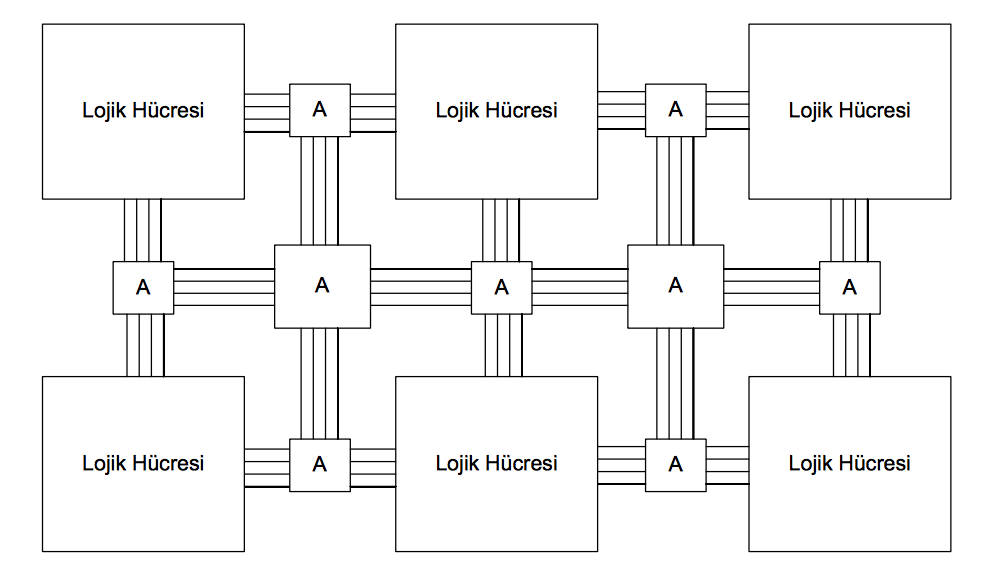
\includegraphics[width=0.8\textwidth]{gorsel/fpgaCLB.png}
%\shorthandoff{=}
%\caption{FPGA Mantık Hücreleri ve Bağlantı Yapısı}
%\label{fpgaCLB}
%\end{figure}

%FPGA'ler esnek mimari yapıları ve programlanma özellikleri sayesinde kendilerine endüstride hızla yer bulmuşlardır ve günümüzde de otomotivden, telekomünikasyona, uzay uygulamalarından savunma sanayine ve özellikle yüksek performansla birlikte esneklik isteyen birçok uygulama alanında tercih edilmektedirler.\par
Xilinx ve Altera firmaları dünya üzerinde en çok müşteriye sahip iki firmadırlar. Bu firmalar birçok uygulamaya özel ve farklı ihtiyaçlara hitap eden değişik FPGA aileleri üretmektedirler. Xilinx firmasının piyasada sıklıkla kullanılan farklı FPGA ailelerinden FPGA örnekleri ve özellikleri tablo \ref{table:fpgaModels}’de verilmiştir.
\begin{longtable}{p{100pt} p{250pt}}
\caption{Xilinx FPGA Kaynak Durumları} \label{table:fpgaModels} \\
\multicolumn{1}{c}{} & 
\multicolumn{1}{c}{\textbf{Logic Slice}} & 
\multicolumn{1}{c}{\textbf{Block RAM (kb)}} &
\multicolumn{1}{c}{\textbf{DSP Slice}} & 
\multicolumn{1}{c}{\textbf{User I/O}} &
\\ 
\hline 
\endfirsthead

\multicolumn{2}{c}%
{{\bfseries \tablename\ \thetable{} -- devam}} \\
\multicolumn{1}{c}{} & 
\multicolumn{1}{c}{\textbf{Logic Slice}} & 
\multicolumn{1}{c}{\textbf{Block RAM (kb)}} &
\multicolumn{1}{c}{\textbf{DSP Slice}} & 
\multicolumn{1}{c}{\textbf{User I/O}} &
\\  \hline 
\endhead

\hline \multicolumn{2}{r}{{Sonraki sayfada devam etmektedir.}} \\ 
\endfoot

\hline \hline
\endlastfoot
  Spartan-3A CX3S200A  &   4032 &   288 &  16  &  248 \\
  Spartan-3A CX3S1400A &  25344 &   576 &  32  &  502 \\
  Virtex-5 XC5VLX50    &   9600 &  1152 &  32  &  400 \\
  Virtex-5 XC5VLX330   & 103680 & 10368 &  192 & 1200 \\
  Virtex-7 XC7V585T    & 182100 & 28620 & 1260 &  850 \\
  Virtex-7 XC7V2000T   & 305400 & 46512 & 2160 & 1200 \\
\end{longtable}

Mantık hücresi (Logic Slice) olarak isimlendirilen birimler FPGA’lerin temel işlem ve depolama birimlerini içermektedirler. Bir mantık hücresinin içerisinde temel olarak 4 ya da daha fazla girişli lookup table (LUT), bir adet flip flop ve çeşitli çoklayıcılar (multiplexer) bulunmaktadır. Basitçe doğruluk tablosu oluşturulabilen sade devreler bir adet mantık hücresi kullanılarak gerçeklenebilir. Fakat karmaşık mantık yapısına ve çokça kaydedici yazmaca (register) ihtiyacı olan devreler ancak birden çok mantık hücresi kullanılarak gerçeklenebilirler. Sürekli gelişmekte olan FPGA teknolojisinde artık FPGA yongalarının içerisine özel fonksiyona sahip makro birimler yerleştirilmektedir. Bu makro birimler hard olarak yongaya gömülü durumda olup sadece izin verilen ölçüde parametreleri programlanabilmektedirler. Bu makro bloklara örnek olarak DCM, RAM, DSP slice, çarpıcı birimleri gösterilebilir. Genel olarak bir FPGA’in mimari yapısı şekil \ref{image:fpgaGenelMimari}’de görülebilir.
\begin{figure}[h]
\centering
\shorthandoff{=}
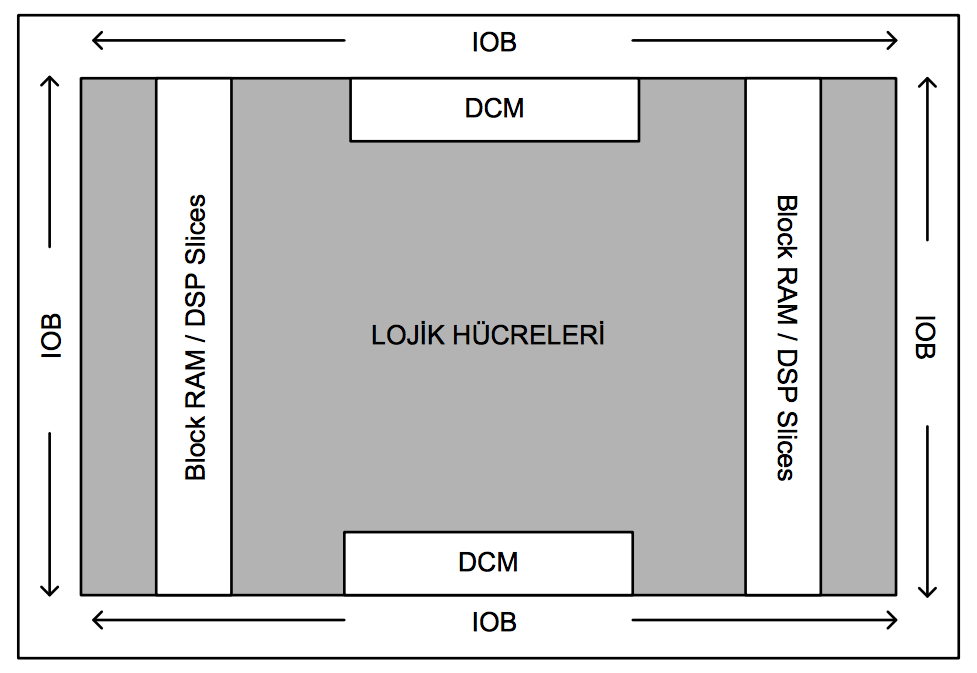
\includegraphics[width=0.8\textwidth]{gorsel/fpgaGenelMimari.png}
\shorthandoff{=}
\caption{FPGA Genel Mimari Yapısı}
\label{fpgaGenelMimari}
\end{figure}
Bu tez çalışması için Xilinx Virtex 7 ailesinden XC7VX690T FPGA’i seçilmiştir. Bu FPGA içinde 108300 slice, 693120 mantık hücresi 866400 CLB flip flop, 10888 KB dağınık ram, 1470 adet 36kbit block ram primitive vardır. \par

\section{GPGPU}

GPU teknolojisindeki ilerlemelerle birlikte, günümüzde kullanılan modern GPU’lar programlanabilir arayüzler sunar hale gelmişlerdir. Bu programlanabilir arayüzler sayesinde GPU’nun işlem gücü ve paralel işleyebilme yeteneği sadece grafik işlemlerinde değil aynı zamanda genel amaçlı hesaplamalarda da kullanılabilir hale gelmiştir. Bu durum ortaya grafik işlem birimi üzerinde genel amaçlı hesaplama (GPGPU - General Purpose programming on Graphic Processing Unit) kavramını çıkarmıştır. \par
GPU’lar yukarıdaki kısımlarda açıklanan işlem hattı mimarisi sayesinde, paralel olarak işlenebilecek nitelikte verinin yüksek performanslı bir şekilde paralel olarak işlenmesi konusunda çok elverişlidirler. GPGPU uygulamaları GPU’ların grafik aygıtlarına özel olan köşe kenar dönüşümü, dokulandırma, renklendirme, gölgelendirme vb. özelliklerinden ziyade SIMD şeklinde çalışan işlem hattı mimarisinden yararlanırlar. GPGPU uygulamaları genel olarak; işaret işleme, ses işleme, görüntü işleme, şifreleme, bioinformatik, yapay sinir ağları, paralelleştirilebilen bilimsel hesaplamalar, istatiksel hesaplamalar gibi yüklü miktarda verinin küçük parçaları üzerinde bağımsız ve paralel olarak işlem yapılmasına uygun olan uygulama alanlarında başarılıdırlar.\par

GPGPU uygulamaları genel olarak CPU üzerinde çalışan bir host program ve GPU’daki çekirdekler üzerinde hesaplama yapacak olaran çekirdek fonksiyonundan (kernel function) oluşur. Her çekirdekte çalışan çerkirdek fonksiyonu, stream şekilde GPU’ya iletilen verinin kendine düşen daha küçük bir birimi üzerinde işlem yapar. Giriş verisinin GPU’ya iletilmesi, sonuç verisinin toplanması istenilen formata dönüştürülmesi gibi ardışık işlemleri CPU’da çalışan host program yürütür. \par
şekil \ref{cudaProgrammingStructure}’da modern GPGPU dillerinden CUDA programlama diline ait programlama modeli yapısı \cite{cudaProgrammingStructure},  tablo \ref{table:cudaCComparision}’de ise C programlama diliyle yazılmış CPU üzerinde çalışan bir matris toplama fonksiyonu ile yine aynı matris toplama fonksiyonunu GPU üzerinde gerçekleyen, CUDA programlama diliyle yazılmış GPU üzerinde çalışan bir kernel fonksiyonu ve C’de yazılmış bir host program gösterilmiştir. şekil \ref{cudaProgrammingStructure}’da görüldüğü üzere, CUDA programlama modelinde GPU aygıtı grid olarak görülür ve çok sayıda bloktan oluşur. GPU’da bulunan çok sayıdaki çekirdekten her biri aynı anda bir blok işleyebilir. Bir blok içerisinde paralel olarak çalıştırılabilen çok sayıda thread bulunur. Bu ipliklerinin her biri kendisine düşen veri öbeği üzerinde tanımlanmış olan çekirdek fonksiyonu çalıştırır.

\begin{figure}[h]
\centering
\shorthandoff{=}
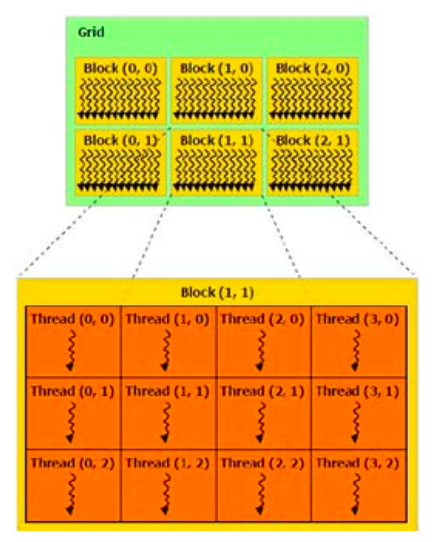
\includegraphics[width=0.8\textwidth]{gorsel/cudaProgrammingStructure.png}
\shorthandoff{=}
\caption{CUDA programlama modeli}
\label{cudaProgrammingStructure}
\end{figure}

\begin{longtable}{p{100pt} p{250pt}}
\caption{Matris Toplama İşleminin C ve CUDA'da Gerçeklenmesi} \label{table:cudaCComparision} \\
\multicolumn{1}{c}{\textbf{CPU C Programı}} & \multicolumn{1}{c}{\textbf{CUDA C Programı}} \\ 
\hline 
\endfirsthead

\multicolumn{2}{c}%
{{\bfseries \tablename\ \thetable{} -- devam}} \\
\multicolumn{1}{c}{\textbf{CPU C Programı}} & \multicolumn{1}{c}{\textbf{CUDA C Programı}} \\ 
\hline 
\endhead

\hline \multicolumn{2}{r}{{Sonraki sayfada devam etmektedir.}} \\ 
\endfoot

\hline \hline
\endlastfoot
  void add_matrix_cpu (float *a, float *b, float *c, int N){  & _global_ void add_matrix_gpu (float *a, float *b, float *c, int N){ \\
    int i,j,index;                                            & int i = blockIdx.x*blockDim.x+threadIdx.x; \\
    for (i = 0 ; i < N ; i++){                                & int y = blockIdx.y*blockDim.y+threadIdx.y; \\
      for (j = 0 ; j < N ; j++){                              & int index = j+i*N; \\
        index = j+i*N;                                        & if (i<N && j<N)  \\
        c[index] = a[index] + b[index];                       &  c[index] = a[index] + b[index]; \\
      }                                                       &} \\
    } & \\
  } & \\
  & \\
  void main(){                    &  void main () { \\
    ...                           &  dim3 dimBlock(blocksize,blocksize);  \\
    add_matrix (a,b,c,N);         &  dim3 dimGrid(N/dimBlock.x,N/dimBlock.y);  \\
    ...                           &  add_matrix_gpu << dimGrid , dimBlock >> (a,b,c,N); \\
  } & }\\
\end{longtable}

Tablo \ref{table:cudaCComparision}’de görüldüğü gibi C programlama dilinde yazılmış olan matris toplama fonksiyonu matris elemanları üzerinde ardışık döngüler şeklinde işlem yaparak matris toplama işlemini gerçekleştirir. CUDA ile yazılmış matris toplama programına bakıldığında, program CPU üzerinde çalışan host programdaki main fonksiyonundan ve GPU üzerinde çalışan add_matrix_gpu çekirdek fonksiyonundan oluşur. Host program bir bloğun boyutunu ve grid içerisindeki blok sayısını belirler. Daha sonra bloklar üzerinde paralel olarak çalışacak olan add_matrix_gpu fonksiyonunu çağırır. çağrı sonucu add_matrix_gpu çekirdek fonksiyonu bloklar ve bloklardaki threadler üzerinde paralel olarak yürütülür. Her bir thread kendi thread numarası (thread ID), blok numarası (block ID) ve blok boyutunu (blockDim) kullanarak kendine düşen veri parçası için matris toplama işlemini gerçekleştirir. \par



\chapter{GEREKSİNİM ANALİZİ} \label{chapter:gereksinimAnalizi}
OpenCL ve CUDA altyapıları kullanılarak gerçeklenen sinyal işleme uygulamalarının, özelleştirilebilir, milli tasarım bir donanım üzerinde çalıştırılması amacı ile başlatılan projenin gereksinimleri \ref{projeGereksinimleri} Mimari Gereksinimleri başlığı altında sunulmuştur. \ref{basarimEtkenleri} Başarım Etkenleri başlığı altında proje için performans metrikleri belirlenmiş, \ref{fonksiyonlarinGerceklenmesi} Fonksiyonların Gerçeklenmesi başlığı altında, Tablo \ref{table:fonksiyonListesi}: Fonksiyon Listesi Tablosunda verilen fonksiyonların matematiksel ifadeleri ve sayısal sistemler üzerinde gerçekleme algoritmaları sunulmuştur.

\section{Mimari Gereksinimleri} \label{projeGereksinimleri}
 Proje gereksinimleri şu şekildedir: 
\begin{enumerate}
  \item Tasarlanan işlemci çok çekirdekli mimariye sahip olmalıdır.
  \item Tasarlanan işlemcinin buyruk kümesi OpenCL 1.2 desteklemelidir. 
  \item Tüm işlemler 32 bit integer ve floating point sayılar üzerinden yapılmalıdır. Floating point sayılar için IEEE754 standardı kullanılmalıdır.
  \item Tasarım modüler olmalı alt modül sayıları parametrik tanımlanmalı, bütün mimari modülleri özelleştirilebilir olmalıdır. 
  \item Gelecek çalışmalarda tasarlanacak özel hesaplama ipcore modülleri için standart bir arayüzü desteklemelidir.
  \item Tasarım sayısal sinyal işleme uygulamalarında sıklıkla kullanılan ve Tablo \ref{table:fonksiyonListesi} içinde belirtilen fonksiyonları desteklemelidir.
  \item Verilen bir matrisin kopyası oluşturulup kopya üzerinden işlem yapılmalıdır.
  \item Reel sayılar matrisi oluşturulurken bellekte yalnızca reel sayıların sığabileceği bir alan kullanılmalıdır, karmaşık sayılar matrisi oluşturulurken reel ve imajiner kısımlar için ayrı yer ayrılmalıdır.
  \item Satır, sütun veya alt matris üzerinde işlem yapılırken yalnızca ilgili veriler kopyalanmalıdır.
  	
\end{enumerate}

\begin{longtable}{p{80pt} p{250pt}}
\caption[Desteklenmesi beklenen fonksiyon listesi]{Desteklenmesi beklenen fonksiyon listesi} \label{table:fonksiyonListesi} \\
\multicolumn{1}{c}{\textbf{Fonksiyon}} & \multicolumn{1}{c}{\textbf{Açıklama}} \\ 
\hline 
\endfirsthead

\multicolumn{2}{c}%
{{\bfseries \tablename\ \thetable{} -- devam}} \\
\multicolumn{1}{c}{\textbf{Fonksiyon}} &
\multicolumn{1}{c}{\textbf{Açıklama}}  \\ \hline 
\endhead

\hline \multicolumn{2}{r}{{Sonraki sayfada devam etmektedir.}} \\ 
\endfoot

\hline \hline
\endlastfoot
 Toplama 								& İki matrisin eleman eleman toplanması 											\\%math_desc%		& C$_{m,n}$=A$_{m,n}$ + B$_{m,n}$  \\
 												& Matrisin tüm elemanlarına sabit eklenmesi										\\%math_desc% 		& C$_{m,n}$= A$_{m,n}$ + b  \\
 Çıkarma 								& İki matrisin eleman eleman farkı 														\\%math_desc		& C$_{m,n}$= A$_{m,n}$ - B$_{m,n}$ \\
 												& Matrisin tüm elemanlarından sabit çıkarılması 							\\%math_desc		& C$_{m,n}$= A$_{m,n}$ - b\\
 Çarpma									& Matrislerin eleman - eleman çarpımı 												\\%math_desc		& C$_{m,n}$= A$_{m,n}$ * B$_{m,n}$\\
 												& Matris çarpımı 																							\\%math_desc		& C = A x B\\
 												& Matrisin tüm elemanlarının sabit ile çarpımı				 				\\%math_desc		& C$_{m,n}$= A$_{m,n}$ * b\\
 Bölme									& Matrislerin eleman - eleman bölümü 													\\%math_desc		& C$_{m,n}$= A$_{m,n}$ / B$_{m,n}$\\
 												& Matrisin tüm elemanlarının sabite bölümü 						 				\\%math_desc		& C$_{m,n}$= A$_{m,n}$ / b\\
 Elemanların toplamı    & Matrisin satır toplamları 																	\\%math_desc		& C$_{(mx1)}$=sum(A,rows)\\
 												& Matrisin sütun toplamları				 														\\%math_desc		& C$_{(1xn)}$=sum(A,cols)\\
 												& Matrisin tüm elemanlarının toplamı 													\\%math_desc		& C = sum(A)\\
 Max, Min,  						& Her satır için																							\\%math_desc		& \\
 Mean, Median						& Her sütun için																							\\%math_desc		& \\
 												& Matrisin tüm elemanları için																\\%math_desc		& \\
 												& En büyük elemanın ilk indisi																\\%math_desc		& \\
 												& Mutlak en büyük elemanın değeri															\\%math_desc		& \\
 												& Mutlak en büyük elemanın ilk indisi													\\%math_desc	  & \\
 Nokta çarpımı					& İki vektörün nokta çarpımı																	\\%math_desc		& C = V$_{1}$ . V$_{2}$\\
 FFT/IFFT								& Her satırın fourier ve ters fourier dönüşümü								\\%math_desc		& \\
 												& Her sütunun fourier ve ters fourier dönüşümü								\\%math_desc		& \\
 Logaritma							& Her eleman için doğal logaritma hesabı											\\%math_desc		& C$_{m,n}$ = ln(A$_{m,n}$)\\	
 												& Her elemean için 10 tabanında logaritma hesabı							\\%math_desc		& C$_{m,n}$ = log10(A$_{m,n}$)\\
 Üssel fonksiyon				& 10 tabanında eksponansiyel 																	\\%math_desc		& C$_{m,n}$ = 10$^{A_{m,n}}$\\
 												& Doğal tabanda eksponansiyel 																\\%math_desc		& C$_{m,n}$ = e$^{A_{m,n}}$\\ 
 Büyüklüğü  						& Matrisin mutlak büyüklüğü																		\\%math_desc		& C = mag(A, abs)\\ 
 												& Matrisin enerjisi																						\\%math_desc		& C = mag(A, sqr) \\	
 Evrişim 								& Dairesel konvolüsyon (Circular convolution)									\\%math_desc		& C = cconv(A, B, n)\\ 
 												& Doğrusal konvolüsyon (Linear convolution) 									\\%math_desc		& C = conv(A, B, n)\\  
 Eşlenik     						&	Bir matrisin karmaşık eşleniği															\\%math_desc		& C = conj(A)\\
 Transpoz								&	Bir matrisin transpozu																			\\%math_desc		& B = A'\\
 											  &	Bir matrisin eşleniksiz transpozu														\\%math_desc		& B = A.'\\			
 Determinant						& Bir kare matrisin determinantı															\\%math_desc		& C = det(A)\\
 Trigonometrik					& Her eleman için sin/cos/tan değerleri 											\\%math_desc		& \\ 			
 Filtreleme							& Her satırı FIR ve IIR Filtreleme 														\\%math_desc		& \\
 												& Her sütunu FIR ve IIR Filtreleme 														\\%math_desc		& \\
 Windowing 							& Hamming, Hanning ve Gaussian 																\\%math_desc		& \\
 Alt matris 						& Matrisin bir satırını al / değiştir   											\\%math_desc		& \\
 												& Matrisin bir sütununu al / değiştir													\\%math_desc		& \\
 												& Matrisin bir alt matrisini al / değiştir										\\%math_desc		& \\
 Türev									& Bir vektörün 1. derecede türevi															\\%math_desc		& \\
 Norm 									& Matrisin ve vektörün p. dereceden normu 										\\%math_desc		& \\
 Sıralama 							& Satır sıralama 																							\\%math_desc		& \\
 												& Sütun sıralama 																							\\%math_desc		& \\
 												& Matris sıralama (vektör sıralama gibi) 											\\%math_desc		& \\
 Varyans,								& Satır bazlı 	 																							\\%math_desc		& \\
 Standart 					& Sütun bazlı 	 																							\\%math_desc		& \\
 Sapma												& Matris bazlı 	 																							\\%math_desc		& \\
 İşaret									& Her bir eleman için signum fonksiyonu 											\\%math_desc		& \\
 Flip										& Yatay ve düşey eksende flip 																\\%math_desc		& \\
 Karekök 								& Her eleman için karekök 																		\\%math_desc		& \\
 Reverse 								& Elemanların sırasını tersine çevirir 												\\%math_desc		& \\
 Interpolasyon 					& Lineer interpolasyon 																				\\%math_desc		& \\
 Karşılaştırma 					& Satır, sütun bazlı veya matris için karşılaştırma 					\\%math_desc		& 
\end{longtable}

Tasarlanan donanımın temel tasarım kararlarını oluşturan gereksinimler ve fonksiyon listesi incelenmiş, her bir matematiksel işlem için gerekli buyruklar ve donanım birimleri belirlenmiştir. 


\section{Başarım Etkenleri}\label{basarimEtkenleri}
Tablo \ref{table:fonksiyonListesi} içinde belirtilen işlemlerin paralelleştirilmesi ile işlem sürelerinin kısalması beklenmektedir. Paralel hesaplamada işlem süresini belirleyen 4 unsur vardır. \par

Bunlardan birincisi bellek işlemlerine ayrılan süredir. Programlanabilir her sistemde olduğu gibi bir işlem veya işlem dizisi başlarken bellekten veri okunur, sonlandığında ise tekrar belleğe sonuçlar yazılır. İşlemler paralelleştirilse de paralelleştirilmese de bellek için harcanan süre toplamda yakındır. Hem yazılım hem de donanım seviyesinde bellek işlemlerinde yerelliği artırmak bellek işlemlerinin daha hızlı işlenmesine olanak sağlar.\par

İkinci unsur paralelleştirmenin bir ölçüsü olan thread sayısıdır. Söz konusu işlem birbirinden bağımsız iş parçacıklarına bölünür ve her bir iş parçacığı farklı donanımlarda koşturularak paralel işleme sağlanır. Literatürde bu iş parçacıkları ingilizce ismi olan thread kelimesiyle ifade edilmekte ve thread kelimesinin buradaki anlamını taşıyan bir türkçe tercümesi bulunmamaktadır. Bu sebeple tezin devamında sürekli olarak thread kelimesi kullanılacaktır. Thread sayısındaki artış, programın daha paralel koşturulabilmesine olanak sağlar.\par

Üçüncü unsur donanımda gerçeklenmiş thread yolu sayısıdır. Her bir thread, bir thread yoluna atanır ve o yol üzerinde koşturulur. Eğer thread yolu sayısı thread sayısından büyük veya eşitse, tek seferde bütün threadler işlenir ve program sonlanır. Eğer thread sayısı, thread yolu sayısından fazla ise threadler, thread yolu sayısı kadar elemana sahip kümelere bölünür. NVidia'nın dokümanlarında warp ismi ile anılan bu thread kümelerinin her biri tek seferde işlenir. Toplam işlem süresi ise warp sayısına bağlı olarak artar. Thread yolu sayısının artırılması warp sayısında ve işlem süresinde azalmaya yol açar. Ancak fiziksel kısıtlardan dolayı thread yolu sayısının bir üst limiti vardır. \par

Dördüncü unsur ise her bir thread için harcanan yürütme zamanıdır. Thread başına düşen yürütme zamanı thread içindeki buyruk sayısına, buyrukların çevrim sayılarına, buyruklar arası veri bağımlılıklarına, işlemcinin boru hattı mimarisine ve işlemcinin frekansına bağlı olarak değişir.\par

Dolayısıyla paralelleştirilmiş bir uygulamanın yürütme zamanı denklem \ref{equation:yurutmeZamani}'de gösterildiği şekilde formüle dökülebilir.

\begin{equation} \label{equation:yurutmeZamani}
t_{program} = t_{bellek} + t_{thread} x \frac{N_{thread}}{N_{thread yolu}} \& 
t_{thread} = N_{buyruk} x c_{ortalama} x T_{saat}
\end{equation} 

Burada $t_{program}$ program süresini, $t_{bellek}$ bellek işlemleri süresini, $t_{thread}$ thread süresini, $N_{thread}$ toplam thread sayısını, $N_{thread yolu}$ toplam thread yolu sayısını, $N_{buyruk}$ thread içindeki buyruk sayısını, $c_{ortalama}$ her buyruk için harcanan çevrim sayılarının ortalamasını, $T_{saat}$ işlemci saatinin periyodunu ifade eder.\par

Thread yolu sayısının 1 olduğu durumda aynı anda tek bir thread işlenebilir. Dolayısıyla işlem paralelleştirilmemiş olur. Thread yolu sayısının sonsuza gitmesi halinde ise program süresi bellek işlemleri için harcanan zamana eşit olur. \par
\textbf{Program süresi bileşenlerinin optimize edilmesi}\par
Thread sayısı ve thread içindeki buyruk sayısı yazılım katmanında belirlenen değerlerdir. Bellek işlemleri için harcanan süre kaçınılmaz olmasına rağmen yazmaç öbeği, paylaşımlı bellek ve ana bellek ara yüzü gibi load ve store işlemleri ile ilgili donanımların tasarımlarında yapılan iyileştirmeler bellek için harcanan süreyi azaltabilir. Öte yandan işlemci frekansı ve işlemler için harcanan ortalama çevrim sayıları da hesaplama işlemlerinin süresini doğrudan belirleyen bileşenler olup optimize edilmesi gerekmektedir. Bu tarz bir optimizasyon için buyruk kümesi ve boru hattı mimarisi belirleyici yapılardır. Buyruk kümesi tasarımı için fonksiyon listesinde bulunan işlemler \par 

\section{Fonksiyonların Gerçeklenmesi} \label{fonksiyonlarinGerceklenmesi}
Fonksiyon listesinde belirtilen fonksiyonların tamamında veriler bellekten okunmakta ve sonuçlar yine belleğe yazılmaktadır. Dolayısıyla load ve store işlemleri fonksiyonlrın tümünde olmalıdır. Her bir fonksiyon için gerekli buyruklar ise her fonksiyonun kendi başlığı altında belirtilmiştir.

\subsection{Toplama işlemi}
İki matrisin eleman eleman toplamında her bir thread $C_{i,j} = A_{i,j} + B_{i,j}$ işlemini yapar. Bu işlem için ihtiyaç duyulan buyruklar floating point ve integer toplama buyruklarıdır. Bir matrisin sabit sayı ile toplanması durumunda ise her bir thread $C_{i,j} = A_{i,j} + k$ işlemini yapar. Burada k değeri integer veya floating point bir sayı olup, bellekten okunabileceği gibi anlık olarak da verilebilir. Dolayısıyla önceki buyruklara ek olarak integer ve float için anlık değer ile toplama buyrukları da gereklidir.

\subsection{Çıkarma işlemi}
İki matrisin eleman eleman toplamında her bir thread $C_{i,j} = A_{i,j} - B_{i,j}$ işlemini yapar. Bu işlem için ihtiyaç duyulan buyruklar floating point ve integer çıkarma buyruklarıdır. Bir matristen sabit sayının çıkarılması durumunda ise her bir thread $C_{i,j} = A_{i,j} - k$ işlemini yapar. Burada k değeri integer veya floating point bir sayı olup, bellekten okunabileceği gibi anlık olarak da verilebilir. Dolayısıyla önceki buyruklara ek olarak integer ve float için anlık değer çıkarma buyrukları da gereklidir.

\subsection{Çarpma işlemi}
MxN ve NxP büyüklükteki iki matrisin çarpılması işlemi MxP adet sonuç üretir. Bu sonuçların her biri için bir thread oluşturulur (toplamda MxP adet) ve her bir thread $C_{i,j} = \sum_{n=0}^{N} (A_{i,n} x B_{n,j})$ işlemini yapar. Bu işlem bir döngü içinde çarpma ve toplama yapılması ile gerçeklenir. Dolayısıyla döngü oluşturabilmek için gerekli atlama, karşılaştırma ve dallanma buyrukları gereklidir. Hesaplama için çarpma buyruğuna da ihtiyaç vardır. Bu işlemin gerçeklenmesinde performans artırmaya yönelik DSP uygulamalarında sıklıkla kullanılan çarp-topla (muladd) işlemi kullanılmalıdır.\par
Matrislerin eleman eleman çarpılması işleminde ise oluşturulan her bir thread $C_{i,j} = A_{i,j} x B_{i,j}$ işlemini yapar. Bu işlem için herhangi bir döngü yapısına ihtiyaç kalmaksızın çarpma buyruğu yeterlidir.\par
Matrisin tüm elemanlarının sabit bir sayı ile çarpılması işleminde her bir thread $C_{i,j} = A_{i,j} / k$ işlemini yapar. Burada k sayısının anlık alınması istenirse anlık ile çarpma buyruğuna da ihtiyaç duyulur.  Bütün çarpma ve çarp-topla buyruklarının float ve integer için versiyonlarının bulunması gerekir.

\subsection{Bölme işlemi}
İki matris arasında eleman-eleman bölme işlemi için oluşturulan her bir thread $C_{i,j} = A_{i,j} / B_{i,j}$ işlemini yapar. Bu işlem için float ve integer bölme buyrukları gereklidir. Bir matrisin sabit sayıya bölümü işleminde ise her bir thread $C_{i,j} = A_{i,j} / k$ işlemini yapar. Burada k sayısının anlık alınması istenirse anlık değere bölme buyruğunun gerçeklenmesi gerekir.

\subsection{Toplam işlemi}
Bir matrisin satır toplamlarını, sütun toplamlarını veya tüm elemanların toplamını bulur. Bütün program ikişerli eleman toplamlarından oluşur. Örneğin tüm satır toplamları için satır başına $log_{2}N$ kez, sütun toplamları için sütun başına $log_{2}M$ kez ardışık toplama işlemi yapılması gerekir. Tüm elemanların toplamı içinse $log_{2}(MxN)$ kez ardışık toplama işlemi yapmak gerekir. İhtiyaç duyulan buyruk ise toplama buyruğudur. 

\subsection{Max,Min,Ortalama,Ortanca, Karşılaştırma}
Verilen herhangi N elemanlı bir veri seti üzerinde (matris veya matrisin bir parçası) max ve min hesapları için ardışık $log_{2}N$ adet karşılaştırma işlemi yapılır. Ortalama hesabı için elemanların toplamı bulunup bölme işlemi yapılır. Ortanca hesabı için ise sıralama yapılması gerekmektedir. Merge-sort algoritması düşünülürse, $log_{2}N$ ardışık karşılaştırma ile sıralama yapılır ve ortanca terim bulunur. Bu fonksiyonlar için öncekilerden farklı olarak karşılaştırma buyrukları gereklidir. 

\subsection{Nokta çarpımı}
$v_{1}$ ve $v_{2}$ iki adet N elemanlı vektör olsun $v_{1} . v_{2} = \sum_{i=1}^{N} v_{1}[i] x v_{2}[i]$ şeklinde tanımlıdır. Daha önce matris çarpımında belirtildiği şekilde çarp, çarp-topla ve topla buyrukları kullanılarak bu işlem gerçekleştirilir. Burada her bir çarpımı oluşturmak için ayrı bir thread oluşturularak paralellik sağlanabilir.

\subsection{FFT/IFFT}
Ayrık zamanda Fourier ve Ters Fourier dönüşümü için günümüzde yaygın olarak kullanılan algoritma Cooley-Tukey FFT algoritmasıdır. \cite{cooleyTukey} Bu algoritmanın radix-2 decimation in time gerçeklemesinin uygulanması durumunda her bir thread bir butterfly işlemini çalıştırır. 8 elemanlı bir vektörün FFT işlemi Şekil \ref{image:fft_radix2_8p}'de sunulmuştur. \par

Fourier transformu alınacak olan giriş sinyali x(n), bu sinyalin fourier transformu ise X(n) olsun.
Radix-2 yönteminde x(n) vektörünün elemanları tek indisli elemanlar ve çift indisli elemanlar olarak ayrılıp, ikişerli gruplara bölünürler. Daha sonra her bir eleman kendinden N/2 uzaktaki eleman ile butterfly işlemine alınır. Şekil \ref{image:fft_radix2_8p}'de sunulan algoritma, Şekil \ref{image:fft_radix2_butterfly}'de çizimi sunulan butterfly işlemlerinden oluşur. Her bir butterfly işleminde yapılan hesaplama denklem \ref{equation:fft_radix2_butterfly}'de gösterildiği gibidir.

\begin{figure}
\centering
\shorthandoff{=}
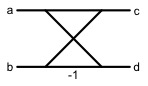
\includegraphics[width=0.3\textwidth]{gorsel/fft_radix2_butterfly.jpg}
\shorthandoff{=}
\caption{Radix 2 için butterfly işlemi}
\label{image:fft_radix2_butterfly}
\end{figure}

$k_{1} = cos(-\frac{2pi}{N})$  $k_{2} = sin(-\frac{2pi}{N})$ \par
\begin{equation} \label{equation:fft_radix2_butterfly}
  \begin{bmatrix}
    c_{Re} & c_{Im} \\[0.3em]
    d_{Re} & d_{Im} 
  \end{bmatrix} 
  = 
  \begin{bmatrix}
    a_{Re} & a_{Im} \\[0.3em]
    a_{Re} & a_{Im} 
  \end{bmatrix}
  +
  \begin{bmatrix}
    b_{Re} & b_{Re} \\[0.3em]
    -b_{Re} & -b_{Re} 
  \end{bmatrix}
  \begin{bmatrix}
    k_{1} \\[0.3em]
    k_{2} 
  \end{bmatrix}
  +
  \begin{bmatrix}
    -b_{Im} & b_{Im} \\[0.3em]
    b_{Im} & -b_{Im} 
  \end{bmatrix}
  \begin{bmatrix}
    k_{2} \\[0.3em]
    k_{1} 
  \end{bmatrix}
\end{equation} 

\begin{figure}[h]
\centering
\shorthandoff{=}
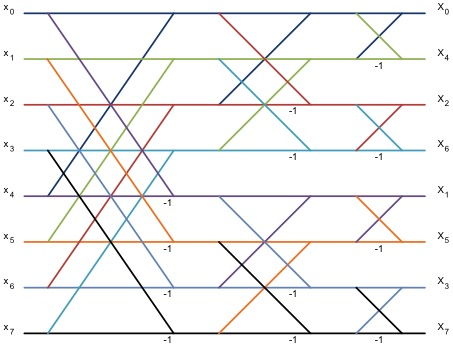
\includegraphics[width=0.8\textwidth]{gorsel/fft_radix2_8p.jpg}
\shorthandoff{=}
\caption{8 noktalı sinyal için FFT Radix 2 algoritması}
\label{image:fft_radix2_8p}
\end{figure}
Denklem \ref{equation:fft_radix2_butterfly}'de görüldüğü üzere her bir butterfly işlemi matris çarpımları ve matris toplamları şeklinde ifade edilebilir. İşleme alınan parametreler a ve b sayılarının reel ve imajiner kısımlarının yanı sıra $sin(-2\pi/N)$ ve $cos(-2\pi/N)$ değerleridir. Burada N değeri sonuç vektörünün her bir elemanın indisi olup, bir eleman için bir kez hesaplanır. \par
FFT gerçeklemesi için sin ve cos değerlerinin hesaplanabilmesi gerekmektedir. Dolayısıyla matris çarpma ve toplama işlemlerinin yanı sıra trigonometri buyrukları da gerekmektedir.

\subsection{Logaritma}
Verilen bir veri setinin her elemanı için doğal logaritma (e tabanında) ve 10 tabanında logaritma hesaplanması gerekir. Xilinx tarafından sağlanan IPCore ile doğal logaritma hızlı bir şekilde hesaplanabilmektedir. 
$log_{a}(x) = log_{e}(x) / log_{e}(a)$ 
denkliğinden faydalanılarak herhangi tabanda logaritma hesaplanabilir. Burada buyruk kümesine $log_{e}x$ buyruğunun da eklenmesi gerekir.

\subsection{Üssel Fonksiyon}
Verilen bir veri setinin her elemanı için $10^{x}$ ve $e^{x}$ değerlerinin hesaplanması gerekir. Xilinx tarafından sağlanan IPCore ile $e^{x}$ hızlı bir şekilde hesaplanabilmektedir. $a^{b} = e^{b x log_{e}{a}}$ denkliğinden faydalanılarak herhangi $a^{x}$ değeri hesaplanabilir.

\subsection{Norm}
Sinyal işlemede yaygınlıkla kullanılan matris normları 1, 2 ve $\infty$ normlardır. 1-norm sütun toplamlarının maksimumu şeklinde tanımlıdır. 
$\|X\|_{1} = max_{j}(\sum_{i}(a_{ij}))$ 2-norm matrisin karesinin en büyük özdeğerinin karekökü olarak tanımlanmıştır. $\|X\|_{2} = \sqrt[2]{max(eig(AxA))}$. Bir matrisin $\infty$ normu ise satır toplamlarının maksimumu olarak tanımlanmıştır. $\|X\|_{\infty} = max_{i}(\sum_{j}(a_{ij}))$.\cite{smith1997matlab}\par
2-norm için kullanılacak özdeğerlerin hesaplanması bu işlemin bir alt parçasıdır. Özdeğer hesaplama algoritmasının gerçeklenmesinde matris büyüklüğü sabit kabul edilemeyeceği ve toplama ve kaydırma gibi temel işlemler cinsinden paralelleştirilebilir bir program yazılabileceği için özdeğer hesaplama işini yazılım seviyesinde gerçeklemek daha uygundur.\cite{eigenvalueComputation} \par

\subsection{Evrişim}
Evrişim (ing. convolution) sinyal işlemede sıklıkla kullanılan bir işlemdir. İki vektörün evrişimi $Conv(f,g)[n]=\sum_{m=-\infty}^{\infty}(f[n]xg[n-m])$ şeklinde hesaplanır. Formülden de anlaşılacağı üzere evrişim sonuç vektörünün her bir elemanı bir dizi çarpımın toplamı şeklinde hesaplanır. Burada sonuç vektörünün her bir elemanı için ayrı thread koşturulursa, 1 çarp ve N-1 çarp-topla buyruğu ile sonuç hesaplanmış olur. 

\subsection{Alt Matris, Flip, Reverse, Eşlenik ve Transpoz}
Karmaşık sayılar düzleminde a + ib şeklinde tanımlanan bir karmaşık sayının eşleniği a - ib sayısıdır. Sayısal sistemlerde karmaşık bir sayının reel ve imajiner kısımları ayrı değerler olarak tutulduğundan imajiner kısmın işaretinin değiştirilmesi eşlenik hesaplaması için yeterlidir. Transpoz işlemi ise matris elemanlarının yerlerinin değiştirilmesi yani okunup işlem yapılmadan yazılması ile gerçeklenir. Alt matris, flip ve reverse işlemleri ise yalnızca okuma ve yazma bellek işlemlerinden oluşur. 

\subsection{Determinant}
Genel geçer determinant hesaplama yönteminde matris, 2x2 boyutunda alt parçalarına ayrılır determinantlarından yeni bir matris oluşturulur, oluşan matris üzerinde yine aynı işlem uygulanır. En son tek elemana düştüğünde matrisin determinantı hesaplanmış olur. 2x2 matrisin determinantı $det(A) = a_{00} x a_{11} + a_{01} x a_{10}$ şeklinde hesaplanır. Bu işlem 1 çarpma 1 çarp-topla buyruğu ile gerçeklenebilir.

\subsection{Trigonometrik İşlemler}
Tüm trigonometrik işlemler sin ve cos cinsinden ifade edilebilir. FPGA platformunda Xilinx IPCore kullanılarak sin ve cos işlemleri hızlıca hesaplanabilir. 

\subsection{Filtreleme ve Windowing}
Filtreleme ve windowing işleminde önceden belirlenmiş bir vektör veya matris işleme alınacak vektör yada matris üzerinde gezdirilerek eleman eleman çarpma ve toplama işlemleri yapılır. Gereksinimlerde belirtilen Hamming Hanning Gaussian windowing işlemlerinde window değişir, işlem aynıdır. FIR ve IIR filtrede de temel işlemler windowing ile aynı olup, algoritma seviyesinde farklılıklar ile gerçeklenir. Bir f vektörü üzerine uygulanacak g maskesi ile filtreleme veya windowing $y[n] = \sum_{i=0}^{N}f[i]xg[i]$ şeklinde gösterilebilir. 

\subsection{Türev}
Bir vektörün türevi, ayrık zamanda ardışık elemanların farkı şeklinde tanımlıdır. N elemanlı bir vektörün türevinin hesaplanması için N adet thread oluşturulur ve her bir thread bir çıkarma işlemi yapar. 

\subsection{Sıralama}
Satır, sütun ve matris elemanlarının sıralanması uygulaması herhangi bir sıralama algoritması ile gerçeklenebilir. Alt seviyede her bir thread  basit karşılaştırma işlemleri yapar.

\subsection{Varyans ve Standart Sapma}
Varyans ve standart sapma için dizinin ortalaması hesaplanır, elemanların ortalamaya uzaklıkları üzerinden toplama, karesini alma ve karekök alma gibi işlemler yapılır. 

\subsection{Karekök}
Karekök işlemi kendi başına bir uygulama olarak değil diğer uygulamaların içinde bir işlem olarak kendini gösterir. Xilinx IPCore kullanılarak karekök işlemi hızlı bir şekilde yapılabildiğinden IPCore kullanımı tercih edilmiştir.

\subsection{İşaret}
İşaret fonksiyonu bir matris veya vektörün tüm elemanları için eleman pozitif ise 1, 0 ise 0, negatif ise -1 değerini döndürür. Eleman sayısı adetinde thread oluşturularak hızlı bir şekilde bu işlem gerçekleştirilebilir.

\subsection{Interpolasyon}
Interpolasyon işlemi, ardışık elemanların ağırlıklı ortalamalalarının hesaplanması ile gerçeklenir. Temel toplama, çarpma, kaydırma, bölme gibi işlemler ile ağırlıklı ortalama hesaplanır. Eleman sayısı kadar thread oluşturularak işlem paralelleştirilebilir.

\subsection{Özet}
Listedeki fonksiyonların incelenmesi ile gerekli hesaplama buyrukları çıkarılmıştır. Fonksiyon listesinin gerçeklenebilmesi için gerekli buyruklar Tablo \ref{table:instructionList1}'de sunulmuştur. 

\begin{longtable}{p{100pt} p{250pt}}
\caption{Gerekli Hesaplama Buyrukları} \label{table:instructionList1} \\
\multicolumn{1}{c}{\textbf{Fonksiyon}} & \multicolumn{1}{c}{\textbf{Açıklama}} \\ 
\hline 
\endfirsthead

\multicolumn{2}{c}%
{{\bfseries \tablename\ \thetable{} -- devam}} \\
\multicolumn{1}{c}{\textbf{Buyruk}} &
\multicolumn{1}{c}{\textbf{Detay}}  \\ \hline 
\endhead

\hline \multicolumn{2}{r}{{Sonraki sayfada devam etmektedir.}} \\ 
\endfoot

\hline \hline
\endlastfoot
  add, addi, fadd     &   Float ve tamsayı değerleri için toplama ve tamsayı için anlık toplama işlemleri \\
  sub, subi, fsub     &   Float ve tamsayı değerleri için çıkarma ve tamsayı için anlık çıkarma işlemleri \\
  mul, muli, fmul     &   Float ve tamsayı değerleri için çarpma ve tamsayı için anlık çarpma işlemleri \\
  div, divi, fdiv     &   Float ve tamsayı değerleri için bölme ve tamsayı için anlık bölme işlemleri \\
  fma, ffma           &   Float ve tamsayı değerler için fused multiply add işlemi \\
  sin, cos, fsin, fcos&   Float ve tamsayı değerler için trigonometrik işlemler \\
  log, flog           &   Float ve tamsayı değerler için e tabanında logaritma işlemi\\
  exp, fexp           &   Float ve tamsayı değerler için $e^{x}$ işlemi \\
  shl, shr, shra      &   Aritmetik ve mantık kaydırma buyrukları \\
  sqrt, fsqrt         &   Float ve tamsayı değerler için karekök işlemi \\
  cmp, br, jump       &   Döngü ve koşul oluşturabilmek için gerekli karşılaştırma, dallanma ve atlama buyrukları \\
\end{longtable}
\chapter{BENZER MİMARİLER VE ÖNCEKİ ÇALIŞMALAR}
Paralel hesaplama için literatürde var olan mimariler Flynn taksonomisi adıyla binilen bir sınıflandırmaya tabidir. Söz konusu donanım, özelliklerine göre bu sınıflandırmada bir sınıfa yerleştirilir. Literatür taramasında öncelikle bu sınıflandırmadan bahsedilmiş, ardından belirlenen sınıfta ön plana çıkan mimariler incelenmiştir.

\section{Paralel işleme taksonomisi}
Bilgisayar bilimlerindeki tüm uygulamalar ve donanımlar paralellik bakımından 4 sınıfta incelenir. Bu sınıflandırma literatürde Flynn Taksonomisi adıyla geçer \cite{flynnTaxonomy}. Literatürdeki kısaltmalarıyla bu 4 sınıf, SISD (Single Instruction Single Data), SIMD (Single Instruction Multiple Data), MISD (Multiple Instruction Single Data) ve MIMD (Multiple Instruction Multiple Data) şeklinde isimlendirilir. 

\begin{figure}
\centering
\shorthandoff{=}
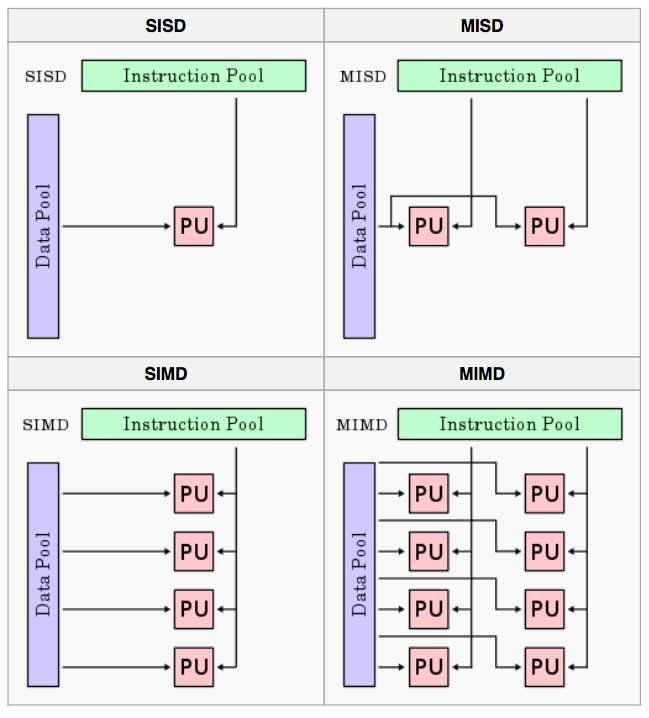
\includegraphics[width=0.9\textwidth]{gorsel/flynnTaxonomy.png}
\shorthandoff{=}
\caption{Flynn Taksonomisi}
\label{overflow}
\end{figure}

SISD mimarilerde herhangi bir paralellikten bahsetmek söz konusu değildir. Tek thread çalıştıran mimariler SISD için örnek olarak gösterilebilir. \par

SIMD mimariler bir buyruğun birden fazla veri seti üzerinde çalıştırıldığı mimarilerdir. Örneğin NxM büyüklüğünde matrislerin toplandığı bir matris toplama işleminde NxM adet veri seti üzerinde basit bir toplama işlemi yapılmaktadır. Gereksinimler ışığında SIMD mimari bu çalışmanın mimari alternatifleri arasındadır. \par

MISD mimariler bir veri seti üzerinde birden fazla buyruğun çalıştırıldığı mimarilerdir. MISD yaygın olarak hata düzelten sistemlerde tercih edilir. Örneğin uzay ortamında çalışması hedeflenen bir hesaplama biriminin ışımalara maruz kalması sebebiyle hesaplamasında veya kaydettiği sonuçlarda yanlışlık olabilir \cite{shivakumar2002modeling}. Bu tarz potansiyel problemlere önlem olarak yapılan her işlem aynı veri seti üzerinde birden fazla kez yapılır ve sonuçlar birden fazla yerde saklanır. Daha sonra aynı verinin kopyaları arasında karşılaştırma yapılırak hatalar algılanır ve düzeltilir. \par

MIMD mimariler bu taksonominin en karmaşık mimarileri olup birden fazla veri seti üzerinde birden fazla buyruğun çalıştırıldığı mimarilerdir. Buna örnek olarak günümüzde kullanılan CPU mimarileri verilebilir. Örneğin Intel Larrabee mimarisi GPU mimarisinde işlevsellik bakımından geliştirilmiş çekirdeklerin kullanılması ile ortaya çıkan bir GPGPU (General Purpose Graphical Processing Unit) olup aynı anda birden fazla veri seti üzerinde birden fazla işlemi koşturabilmektedir \cite{seiler2008larrabee}.\par

Proje gereksinimlerinde ve fonksiyon listesinde belirtilen, hedef donanım hakkındaki ihtiyaçlar, Flynn taksonomisinde SIMD sınıfı ile örtüşmektedir. MIMD bir mimari ise proje gereksinimlerinin üzerinde bir özellik olup, eniyileştirmeye yönelik bir çalışma olabilir.

\section{Mevcut Mimariler}
Gereksinimlerde belirtilen fonksiyonlar ışığında hesaplamalar için kullanılacak modüller belli IPCore donanımları ve basit hesaplama modüllerinden oluşur. Paralel işlemeye özel donanımlarda yürütme zamanının en büyük bileşeni verilerin okunması ve yazılmasından oluşan bellek işlemleri olduğu için mimari seviyesinde donanım özelliklerini belirleyici unsur, veri yolu tasarımıdır.\par

Veri yolu mimarisi, bellek, yazmaç öbekleri ve hesaplama birimleri arasındaki bağlantı ile bu yapıların mimari hiyerarşisinden oluşur. Literatürde öne çıkan veri yolu mimarileri üç sınıfta değerlendirilebilir: Homojen az çekirdekli işlemciler, homojen çok çekirdekli işlemciler ve heterojen yapıdaki işlemciler. \par

\subsection{Homojen az çekirdekli işlemciler}
Homojen az çekirdekli mimariler birbirinin aynı olan az sayıda yüksek işlem kapasiteli çekirdeklerin 2. veya daha üst seviyede önbellekler üzerinden veri paylaşımı sağladığı işlemcilerdir. Bu mimaride her işlemci çekirdeğin kendisine ait bir önbelleği vardır. Bunlar bir interconnect yardımıyla bütünleşik bir paylaşımlı önbelleğe bağlanırlar. Bu yapıya örnek olarak Intel'in Nehalem işlemcisi gösterilebilir \cite{molka2009memory} \cite{hackenberg2009comparing}. Nehalem mimarisinde hususi önbellek 2 seviyeye ayrılmıştır ve paylaşımlı önbellek 3. seviyeyi oluşturmaktadır. Çekirdekler 3. seviye önbelleğin ardından Şekil \ref{image:nehalem}'deki gibi bir bellek denetleyicisi ile sistemin ana belleğine bağlanır.\par

\begin{figure}
\centering
\shorthandoff{=}
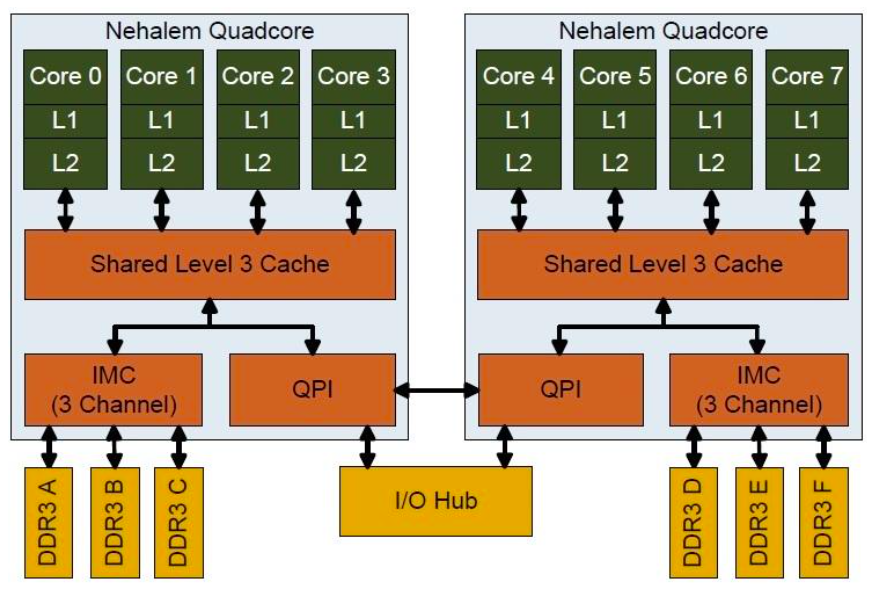
\includegraphics[width=0.9\textwidth]{gorsel/nehalem.jpg}
\shorthandoff{=}
\caption{Intel Nehalem Mimarisi}
\label{image:nehalem}
\end{figure}

\subsection{Homojen çok çekirdekli işlemciler}
Homojen çok çekirdekli mimariler birbirinin aynı olan çok sayıda düşük işlem kapasiteli çekirdeklerden oluşan yapılardır. Bunlara örnek olarak grafik işlemcileri verilebilir \cite{MCSE.2012.23}. Şekil \ref{image:nvidiagpu}'teki gibi bir yapıya sahip olan grafik işlemcilerde amaç, paralelliği ön plana çıkarmak, çok sayıda verinin aynı anda işlenebilmesine olanak sağlamaktır. Az çekirdekli işlemcilerin aksine belleği kullanmak isteyen daha çok çekirdek olacağından bu mimarilerde bellek açısından bir darboğaz oluşmasına sebep olur. Homojen çok çekirdekli mimarilerin bellek hiyerarşisi 2 seviyeli önbellek ve ana bellekten oluşur. Her iki önbellek de çekirdek adacığında paylaşımlıdır. Az çekirdekli mimarilerin aksine çok çekirdekli mimarilerde genel bir yazmaç öbeği tüm çekirdeklerin erişimine açık olup yürütme zamanında her bir çekirdeğe özel olarak atanır.

%\begin{figure}[h] \label{image:nvidiagpu} 
%\centering 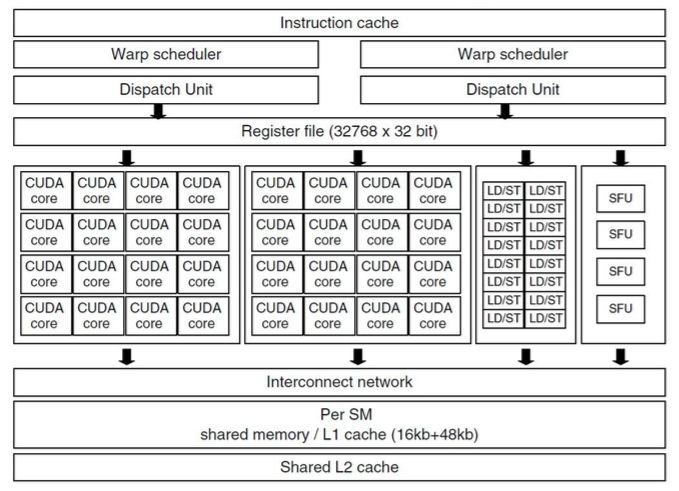
\includegraphics[width=300pt]{gorsel/nvidiagpu.jpg} \caption{Nvidia GPU}  
%\end{figure}

\begin{figure}
\centering
\shorthandoff{=}
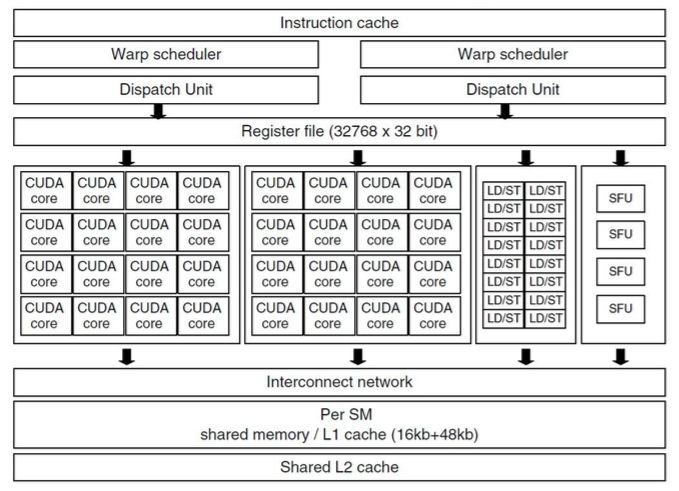
\includegraphics[width=0.9\textwidth]{gorsel/nvidiagpu.jpg}
\shorthandoff{=}
\caption{Nvidia GPU}
\label{image:nvidiagpu}
\end{figure}



Homojen az çekirdekli mimariler genel amaçlı kullanılan CPU (Central Processing Unit) mimarilerinde tercih edilirken çok çekirdekli mimariler GPU (Graphical Processing Unit) ön plana çıkar. CPU çekirdekleri yüksek işlem gücüne sahip ve az sayıda iken GPU çekirdekleri düşük işlem gücüne sahip ve çok sayıdadır. CPU üzerinde koşturulan programların dallanma ve bellek işlemleri için harcadığı zamanın azaltılması için çekirdeklere yakın büyük kapasiteli önbellekler kullanılır. GPU çekirdeklerinin sayıca fazla olması paralel hesaplamayı ön plana çıkarmakta ve ana bellek erişimi için kullanılan veri yolu genişliği, önbellek büyüklüğünden daha önemli bir kriter olmaktadır. Tablo \ref{table:cpuGpuComparision} içinde CPU ve GPU mimarilerinin bellek özellikleri sunulmuştur \cite{cpuGpuMemoryTable}. \par

\begin{longtable}{p{150pt} p{100pt} p{100pt}}
\caption[CPU GPU Bellek Karşılaştırması]{CPU GPU Bellek Karşılaştırması} \label{table:cpuGpuComparision} \\
\multicolumn{1}{c}{} & \multicolumn{1}{c}{\textbf{CPU}} & \multicolumn{1}{c}{\textbf{GPU}} \\ 
\hline 
\endfirsthead

\multicolumn{2}{c}%
{{\bfseries \tablename\ \thetable{} -- devam}} \\
\multicolumn{1}{c}{} & \multicolumn{1}{c}{\textbf{CPU}} & \multicolumn{1}{c}{\textbf{GPU}} \\  
\hline 
\endhead

\hline 
\multicolumn{3}{r}{{Sonraki sayfada devam etmektedir.}} \\ 
\endfoot

\hline \hline
\endlastfoot
  Bellek 									&		 6 -  64 GB 		& 	768 MB - 6 GB 	\\
  Bellek Bant Genişliği 	&		24 -  32 GB/s 	& 	100 - 200 GB/s 	\\
  L2 Önbellek				 			&		 8 -  15 MB 		& 	512 - 768 KB 		\\
  L1 Önbellek				 			&	 256 - 512 KB 		& 	 16 -  48 KB 		\\
\end{longtable}

Homojen çok çekirdekli mimarilere verilebilecek bir örnek de sunucu sistemlerinde kullanılan Tile mimarisidir. \cite{tileArchitecture} Bu mimaride 36-100 arasında RISC işlemciden oluşan çekirdekler birbirlerine bağlanarak yüksek paralellik elde edilir. Tile mimarisinde bellek mimarisi olarak şekil  \ref{image:tileArchitecture}'te sunulan NUCA (non-uniform cache architecture) önbellek mimarisi kullanılır. Bu mimaride çekirdeklerin her birinin kendine ait özel önbelleği vardır. İkinci seviye önbellek olarak diğer çekirdeklerin önbellekleri kullanılır. Örnek olarak, 64 çekirdekli bir işlemcide her bir çekirdeğin 32 KB önbelleği olduğunu varsayarsak; 1 numaralı çekirdeğin 32 KB 1. seviye ve 2016 KB 2. seviye önbelleği olacaktır. Bu tasarımda herhangi bir çekirdeğin diğer tüm çekirdeklerin önbelleklerine bağlantısı olmalıdır. Çekirdek sayısının artması ile bu gereksinim bir wiring problemine dönüşür ve uzun yollar kritik yolu etkileyerek toplam gecikmeye katkıda bulunabilir. Bu kısıttan dolayı Tile mimarisinde 2 boyutlu bir MESH ağı kurulmuş ve her bir çekirdek bu ağdaki bir node olarak yerleştirilmiştir. Her node bir çekirdek, bir önbellek ve bir routerdan oluşur. Bir çekirdek kendinden farklı tüm çekirdeklerin ön belleklerini ikinci seviye ön bellek olarak kullandığından MESH network üzerinden her birine erişimi vardır. Ancak fiziksel olarak kendisine uzak olan veriye erişebilmesi komşuluğundaki routerlar üzerinden her seferinde bir birim şeklindedir. Bu davranış satranç tahtası üzerinde şahın hareketi gibi düşünülebilir. MESH network yapısında tüm verilere erişim hızı aynı olmamakla birlikte, maksimum gecikme, node sayısının karekökü ile orantılı olarak artar. 

\begin{figure}
\centering
\shorthandoff{=}
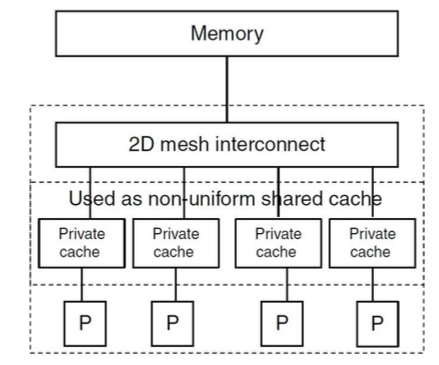
\includegraphics[width=0.9\textwidth]{gorsel/tileArchitecture.png}
\shorthandoff{=}
\caption{Tile Mimarisi}
\label{image:tileArchitecture}
\end{figure}

\subsection{Heterojen yapıdaki işlemciler}
Birbirinin aynı olan çekirdeklerin az veya çok sayıda gerçeklenmesi ile elde edilen paralel hesaplama donanımları çoğu uygulamada performans açısından yeterli gelse de, bir takım uygulamalarda sık kullanılan bazı işlemlerin hızlandırılması adına özel donanımlar gerçeklenir. Literatürde bu tip işlemciler heterojen yapıdaki işlemciler olarak adlandırılır. Heterojen mimariler doğrudan amaca yönelik hazırlandıkları için çok farklı mimari yapılarda gerçeklenebilirler. Heterojen mimarilerin temel özelliği bir işi her zaman o işi en hızlı yapan donanıma vermeleridir. Bu sebeple sık kullanılan hemen her işlem için ayrı hesaplama birimleri yerleştirilerek, özel fonksiyonların yazılım seviyesinden donanım seviyesine indirilmesi sağlanır. Örnek olarak şekil \ref{image:playStationArchitecture}'te sunulan heterojen mimari çizimi Playstation oyun konsollarında kullanılan Cell mimarisine aittir. 


\begin{figure}
\centering
\shorthandoff{=}
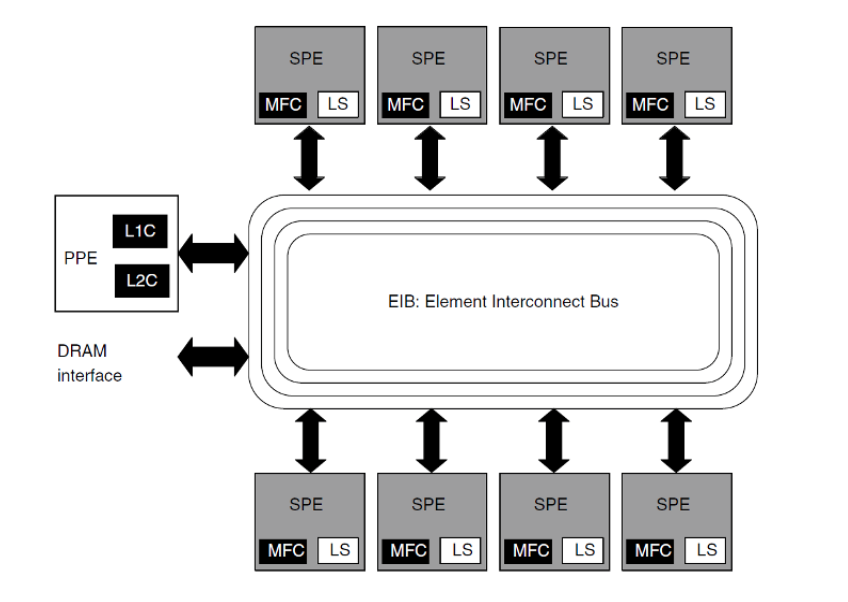
\includegraphics[width=0.9\textwidth]{gorsel/playStationArchitecture.png}
\shorthandoff{=}
\caption{Sony Playstation Cell Mimarisi}
\label{image:playStationArchitecture}
\end{figure}


Şekil \ref{image:playStationArchitecture}'te gösterilen Cell mimarisinde PPE (Power processing element) ana işlemci olup, SPE (Synergistic processing element) bloklarının her biri ise DSP benzeri SIMD işlemcilerdir.
\chapter{GENEL İŞLEMCİ MİMARİSİ}
İşlemci tasarımı buyruk kümesinin tasarlanması ile başlar. Daha sonra buyrukların koşturulabilmesi için gerekli donanımlar belirlenir ve bu donanımların yüksek verimli kullanımını sağlamak için boru hattı mimarisi tasarlanır. Tezin bu bölümünde öncelikli olarak buyruk kümesi mimarisi anlatılacak, ardından her buyruğun ihtiyaç duyduğu hesaplama modülleri belirlenecek, sonrasında kullanım senaryoları üzerinden boru hattı mimarisi tasarımı anlatılacaktır. Son olarak Tosun işlemcisinin veri yolu mimari yapısı ve tasarım kararları üzerinde durulacaktır.\par

\section{Buyruk Kümesi Mimarisi}
Hedeflenen işlemciye benzer özelliklerde mevcut paralel işlemcilerin buyruk kümesi mimarileri incelenmiş, gereksinim analizinde fonksiyonların gerçeklenebilmesi için gerekli olarak belirlenen buyruklar bu buyruk kümesi mimarilerine eklenerek Tosun işlemcisi için bir buyruk kümesi mimarisi oluşturulmuştur. Mevcut buyruk kümelerinin incelenmesinin sebebi paralel işlemcilerin mimari özelliklerinden bağımsız olarak sahip olması gereken ortak özelliklerin bulunmasıdır. Bu özelliklerden bazıları yükleme ve saklama operasyonları, threadler arası senkronizasyonun sağlanması, çekirdeklerin bellek erişimlerinde kullanılan adres hesaplamaları, yazmaçlar üzerinde yapılan okuma ve yazma işlemleridir. \par

Tosun buyruk kümesi mimarisinin oluşturulmasında NVidia PTX \cite{nvidiaPTXISA} buyruk kümesi paralel işleme mimarisi olarak temel alınmıştır. Ayrıca adres hesapları, dallanmalar, temel aritmetik ve mantık işlemleri gibi her işlemcinin sahip olması gereken temel buyruklar için de Intel x86 \cite{x86ISA} ve MIPS \cite{MIPSISA} buyruk kümeleri referans alınmıştır. \par

Tosun buyruk kümesi mimarisinde bulunmasına karar verilen buyruklar tablo \ref{table:tosunInstructions} içinde sunulmuştur. 



\begin{longtable}{p{50pt} p{300pt} p{70pt}}
\caption{Tosun Buyruk Listesi} \label{table:tosunInstructions} \\
\multicolumn{1}{l}{\textbf{Buyruk}} & \multicolumn{1}{l}{\textbf{Açıklama}} & \multicolumn{1}{c}{\textbf{Türü}} \\ 
\hline 
\endfirsthead

\multicolumn{2}{c}%
{{\bfseries \tablename\ \thetable{} -- devam}} \\
\multicolumn{1}{l}{\textbf{Buyruk}} &
\multicolumn{1}{l}{\textbf{Açıklama}} &
\multicolumn{1}{c}{\textbf{Türü}}  \\ \hline 
\endhead

\hline \multicolumn{2}{r}{{Sonraki sayfada devam etmektedir.}} \\ 
\endfoot

\hline \hline
\endlastfoot
  addi		&	 $r_{d} = r_{s1} + 			$anlık 	& \multicolumn{1}{c}{Anlık} 	\\
  andi 		&	 $r_{d} = r_{s1} \& 		$anlık 	& \multicolumn{1}{c}{Anlık}  	\\
  ori 		&	 $r_{d} = r_{s1} | 			$anlık  & \multicolumn{1}{c}{Anlık}  	\\
  xori 		&	 $r_{d} = r_{s1} \oplus $anlık 	& \multicolumn{1}{c}{Anlık}  	\\
  divi 		&	 $r_{d} = r_{s1} / 			$anlık  & \multicolumn{1}{c}{Anlık}  	\\
  muli 		&	 $r_{d} = r_{s1} x 			$anlık  & \multicolumn{1}{c}{Anlık}  	\\
  subi 		&	 $r_{d} = r_{s1} - 			$anlık  & \multicolumn{1}{c}{Anlık}  	\\
  movi 		&	 $r_{d}(alt) = 	$anlık  & \multicolumn{1}{c}{Anlık}  	\\
  movhi		&	 $r_{d}(ust) = 	$anlık  & \multicolumn{1}{c}{Anlık}  	\\
  fabs  	&  $r_{d} = |r_{s1}|			$				&	\multicolumn{1}{c}{Y1}		 	\\
  fadd  	&  $r_{d} = r_{s1} + r_{s2}$			&	\multicolumn{1}{c}{Y2}		 	\\
  fcom  	&  $r_{d} = com(r_{s1},r_{s2})$		&	\multicolumn{1}{c}{Karşılaştırma}	 	\\
  fdiv  	&  $r_{d} = r_{s1} / r_{s2}$			&	\multicolumn{1}{c}{Y2}		 	\\
  fmul  	&  $r_{d} = r_{s1} x r_{s2}$			&	\multicolumn{1}{c}{Y2}		 	\\
  fsqrt  	&  $r_{d} = sqrt(r_{s1})$					&	\multicolumn{1}{c}{Y1}		 	\\
  fcos  	&  $r_{d} = cos(r_{s1})$					&	\multicolumn{1}{c}{Y1}		 	\\
  fsin  	&  $r_{d} = sin(r_{s1})$					&	\multicolumn{1}{c}{Y1}		 	\\
  ffma  	&  $r_{d} = r_{s1}xr_{s2}+r_{s3}$	&	\multicolumn{1}{c}{Y3}		 	\\
  ffms  	&  $r_{d} = r_{s1}xr_{s2}-r_{s3}$	&	\multicolumn{1}{c}{Y3}		 	\\
  fmin  	&  $r_{d} = min(r_{s1},r_{s2})$		&	\multicolumn{1}{c}{Y2}		 	\\
  fmax  	&  $r_{d} = max(r_{s1},r_{s2})$		& \multicolumn{1}{c}{Y2}			\\
  fln 	 	&	 $r_{d} = log_{e}(r_{s1})$			& \multicolumn{1}{c}{Y1}			\\
  fmod 		&	 $r_{d} = r_{s1} \% r_{s2} $ 		& \multicolumn{1}{c}{Y2}  		\\
  f2int 	&	 $r_{d} = r_{s1}$ 							& \multicolumn{1}{c}{Y1}  		\\
  int2f		&	 $r_{d} = r_{s1}$ 							& \multicolumn{1}{c}{Y1}  		\\
  fchs		&	 $r_{d} = -r_{s1}$ 							& \multicolumn{1}{c}{Y1}  		\\
  fexp 		&	 $r_{d} = e^{r_{s1}}$						& \multicolumn{1}{c}{Y1}  		\\
  add 		&	 $r_{d} = r_{s1} + r_{s2}$ 			& \multicolumn{1}{c}{Y2}  		\\
  and 		&	 $r_{d} = r_{s1} \& r_{s2}$ 		& \multicolumn{1}{c}{Y2}  		\\
  or 			&	 $r_{d} = r_{s1} | r_{s2}$			& \multicolumn{1}{c}{Y2}  		\\
  xor			&	 $r_{d} = r_{s1} xor r_{s2}$ 		& \multicolumn{1}{c}{Y2}  		\\
  div  		&  $r_{d}	= r_{s1} / r_{s2}$			&	\multicolumn{1}{c}{Y2}		 	\\
  mul  		&  $r_{d} = r_{s1} x r_{s2}$			&	\multicolumn{1}{c}{Y2}		 	\\
  shl  		&  $r_{d} = r_{s1} << r_{s2}$			&	\multicolumn{1}{c}{Y2}		 	\\
  shr  		&  $r_{d} = r_{s1} >> r_{s2}$			&	\multicolumn{1}{c}{Y2}			\\
  shra  	&  $r_{d} = r_{s1} >> r_{s2}$			&	\multicolumn{1}{c}{Y2}		 	\\
  sub  		&  $r_{d} = r_{s1} - r_{s2}$			&	\multicolumn{1}{c}{Y2}		 	\\
  min  		&  $r_{d} = min(r_{s1},r_{s2})$		&	\multicolumn{1}{c}{Y2}		 	\\
  max  		&  $r_{d} = max(r_{s1},r_{s2})$		&	\multicolumn{1}{c}{Y2}		 	\\
  chs  		&  $r_{d} = -r_{s1}$							&	\multicolumn{1}{c}{Y1}		 	\\
  not  		&  $r_{d} = ~r_{s1}$							&	\multicolumn{1}{c}{Y1}		 	\\
  abs  		&  $r_{d} = |r_{s1}|$							&	\multicolumn{1}{c}{Y1}		 	\\
  com  		&  $r_{d} = com(r_{s1},r_{s2})$		& \multicolumn{1}{c}{C}			\\
  mod  		&  $r_{d} = r_{s1} \% r_{s2})$		& \multicolumn{1}{c}{Y2}			\\
  brv 		&	 Verilen yazmaçtaki bitleri ters sırada hedef yazmaca yazar & \multicolumn{1}{c}{Y1}  \\
  bfr 		&	 Verilen yazmacın belirtilen kadar kısmını maskeleyip hedef yazmaca yazar & \multicolumn{1}{c}{Y1}  \\
  br 			&	 Karşılaştırma bayraklarında belirtilen koşul varsa, verilen adres kadar ileri atlar & \multicolumn{1}{c}{Dallanma}  \\
  fin 		&	 Programı sonlandırır& \multicolumn{1}{c}{Sistem}  \\
  ldshr 	&	 Paylaşımlı bellekten yükleme işlemi yapar& \multicolumn{1}{c}{Y1}  \\
  stshr 	&	 Paylaşımlı belleğe saklama işlemi yapar& \multicolumn{1}{c}{Y1}  \\
  sync		&	 Tüm threadler aynı noktaya gelinceye kadar önce gelen threadleri bekletir. & \multicolumn{1}{c}{Sistem}  \\
  ldram 	&	 Ana bellekten yükleme işlemi yapar& \multicolumn{1}{c}{Y1}  \\
  stram		&	 Ana belleğe saklama işlemi yapar& \multicolumn{1}{c}{Y1}  \\
  mov 		&  $r_{d}$ = $r_{s1}$ 						&	\multicolumn{1}{c}{Taşıma}		 \\
  jmp  		&  Program sayacına belirtilen sayıyı ekleyerek atlar &	\multicolumn{1}{c}{Atlama}		 \\
  
\end{longtable}

Tosun buyruk kümesinde toplam 56 adet buyruk belirlenmiştir. Tablo \ref{table:tosunInstructions} içinde verilen buyruklar içerdikleri işlenen tür ve sayılarına göre türlere ayrılmıştır. Bu sınıflandırma buyruk içinde belirtilmesi gereken işlenen cins ve sayılarına göre yapılmıştır. Buyruk türlerinin bit yapısının belirlenebilmesi için öncelikle buyruk içine yerleştirilecek bilgilerin bit genişlikleri belirlenmelidir. \par

Buyruk bit yapılarında kaynak ve hedef hafıza birimleri olarak yazmaç numaraları kullanılır. Buyruk içinde bir yazmacın kaç bit ile ifade edileceği, bir thread için tahsis edilen yazmaç sayısına bağlıdır. İşlemci mimarisinde yazmaç sayısının belirlenmesi bir ödünleşimli karardır. Yazmaç sayısının artması yazmaçlar için kullanılan alanı artıracağı gibi yazmaç numaraları için kullanılan karşılaştırıcı devrelerin de büyümesine sebep olur. Öte yandan yazmaç sayısının azlığı bellek işlemlerinin artmasına ve başarımın düşmesine sebep olacaktır. Tosun mimarisinde çok çekirdekli bir mimariden söz edildiği için yazmaç sayılarının artışı tek çekirdekli işlemcilere oranla daha fazla bir alan kullanımında artışa sebep olmaktadır. Bu yüzden Tosun mimarisinde hedef programlara yetebilecek minimum sayıda yazmaç kullanılmıştır. Bu çalışmada NVidia CUDA ile çalışan 184 adet paralel hesaplama uygulamasının yazmaç kullanım adetleri incelenmiştir. Elde edilen sonuçlara göre Tablo \ref{table:NVidiaRegisterUsage}'ta sunulduğu şekilde 64 adetten fazla sayıda yazmaç kullanan program ile karşılaşılmamıştır.

\begin{longtable}{p{350pt} p{100pt} }
\caption{NVidia GPGPU Programları Yazmaç Kullanım Analizi} \label{table:NVidiaRegisterUsage} \\
\multicolumn{1}{l}{\textbf{Açıklama}} & \multicolumn{1}{r}{\textbf{Adet}}  \\ 
\hline 
\endfirsthead
32 veya daha az sayıda yazmaç kullanan uygulamalar  & \multicolumn{1}{r}{138} \\
32 ile 64 adet arasında yazmaç kullanan uygulamalar & \multicolumn{1}{r}{46}  \\
64 yazmaçtan fazla sayıda yazmaç kullanan uygulamalar & \multicolumn{1}{r}{0} \\
\end{longtable}

Neticede her bir thread için 64 adet yazmaçtan oluşan yazmaç öbeği kullanılmasına karar verilmiştir. Projenin bir diğer isteği olan OpenCL desteği ise OpenCL spesifikasyonlarında belirtilen bazı özel amaçlı yazmaçların gerçeklenmesini zorunlu kılmaktadır. Lokal thread numarası ve global thread numarası gibi programcının erişimine açık olması gereken ve spesifikasyonda belirtilen bilgiler program içinde özellikle adres hesaplamalarında sıklıkla kullanılmakta olduğundan yazmaç öbeğinde tutulması faydalı olacaktır. Bu bilgilerin yanı sıra program parametrelerinin de yazmaç öbeğine dahil edilmesi ile yazmaç sayısı 128 adete çıkarılmıştır. Ancak 128 yazmacın yalnızca ilk 64 adedi genel amaçlı olup, son 64 adeti özel mov buyruğu ile erişilebilir olarak belirlenmiştir. Toplamda 64 adet genel amaçlı yazmaç, buyruk içinde 6 bit ile ifade edilebilir. \par

Tüm işlemler 32 bit genişliğinde float veya tam sayılar ile yapılmaktadır. Yazmaç sayıları ve işlem kodu da hesaba katıldığında genel olarak buyrukların 32 bit genişliğe sığdırılabileceği hesaplanmıştır. Buyruklar için ayrılan bellek alanının verimli kullanılabilmesi için buyruk genişliklerinin de 32 bitten fazla olmamasına karar verilmiş, bu sebeple de buyruk içinde verilen anlık değerler 16 bit genişliğine sabitlenmiştir. Bir yazmaca anlık bir değerin yazılması ise movi ve movhi buyruklarının peş peşe kullanılması ile mümkündür. \par

\begin{figure}[ht]
\centering
\shorthandoff{=}
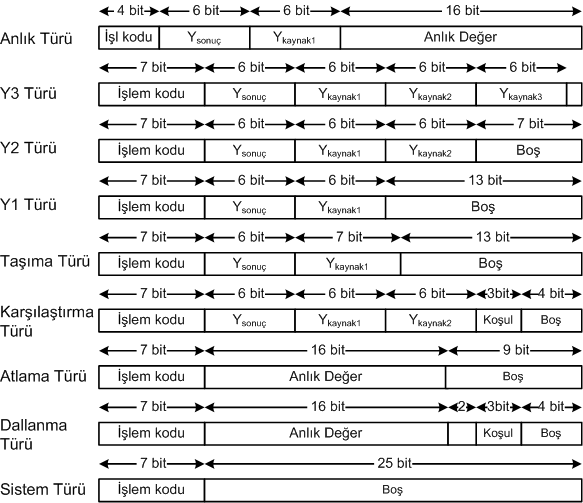
\includegraphics[width=0.9\textwidth]{gorsel/instructionTypes.png}
\shorthandoff{=}
\caption{Tosun Buyruk Türleri}
\label{image:instructionTypes}
\end{figure}

Anlık türü buyruklar bir kaynak yazmacı, bir hedef yazmacı ve bir anlık değer içerir. Dolayısıyla işlem kodu için yalnızca 4 bitlik boş yer kalır. 4 bit, işlem koduna yeterli olmadığı için, olası tasarım çözümleri anlık değerin daraltılması veya buyruk genişliğinin artırılmasıdır. Buyruk genişliğinin değiştirilmesi durumunda bellek yönetimi, buyruk çekme ve kod çözme donanımları karmaşıklaşırken anlık değerin daraltılması durumunda ilave buyruklar gerekeceği gibi, programcının da tasarımı karmaşıklaşmaktadır. Bu probleme özel bir çözüm olarak anlık türü buyrukların 4 bit işlem koduna sahip olmasına karar verilmiştir. Anlık buyruklarda işlem koduna 4 bit ayrılmış olması, işlem kodunun kalan alt bitlerinin x ile doldurulması anlamına gelir. Toplamda 9 adet anlık türü buyruk bulunmaktadır. Dolayısıyla üst 4 biti [0,9] aralığında olan işlem kodları anlık türünde, [10,15] aralığında olan işlem kodları ise diğer türlerdedir. Buyruk kümesinde anlık türü olmayan, 46 adet buyruk vardır. Üst 4 bit için kullanılmayan 6 farklı değer olduğundan alt bitler için 8 farklı değer, dolayısıyla 3 bit gereklidir. \par

Anlık türü buyruklardan kaynaklı bu değişiklik ile Tosun buyrukları 7 bit işlem kodu ile ifade edilir, 0000000 - 1001111 aralığındaki işlem kodları anlık türü buyruklara karşılık gelir, anlık türü buyruklarda alt 3 bit önemsiz olarak kabul edildiğinden yalnızca üst 4 bit buyruk içinde yer alır. Örneğin 0000xxx işlem kodu addi buyruğuna karşılık gelir. Dolayısıyla alt 3 bit buyruğun bit dizisi içinde yer almaz ve gelen herhangi bir buyruk için üst 4 bit 0000 ise buyruğun addi olduğu anlaşılır. Tüm buyruk türlerinin bit yapısı Şekil \ref{image:instructionTypes}'ta sunulmuştur. \par



\section{Hesaplama Modülleri}
Buyruk listesinde her bir buyruk için mimariye eklenmesi gereken hesaplama modülleri irdelenmiş, her bir buyruk için verimin yüksek tutulması adına ilgili optimize edilmiş Xilinx IPCore kullanımına öncelik verilmiştir.\par
\begin{itemize}
\item add, addi, sub, subi, abs, chs buyruklarının hesaplamaları tamsayı toplayıcı ipcore kullanılarak yapılır. Bu işlem birimi hem toplama hem çıkarma işlemini gerçeklemektedir.
\item mul ve muli buyrukları integer çarpma IPCore kullanılarak gerçeklenir.
\item and, andi, or, ori, not, xor, xori, brv ve bfr buyrukları mantıksal bit işlemleri yaparlar. Bu buyrukların her biri için ayrı bir işlem modülü kullanılır.
\item min, max ve com buyrukları için iki sayının karşılaştırılması gerekmektedir. Bu üç buyruk bir karşılaştırıcı modülünü kullanır. Com buyruğu işlem neticesinde büyük, küçük ve eşit bayraklarının değerini değiştirirken min ve max işlemleri sayılardan küçük olanı veya büyük olanı sonuç yazmacına yazar. 
\item div, divi ve mod buyrukları bölme işlemi için hazırlanmış ipcore kullanırlar.  
\item shl, shr, shra buyrukları kaydırıcı modül kullanılarak gerçeklenirler.
\item f2int ve int2f buyrukları float ve integer veri tipleri arasında dönüşüm sağlar. Her ikisi için de hazır IPCore gerçeklenir.
\item fadd ve fsub buyrukları için float toplayıcı IPCore kullanılarak gerçeklenir.
\item fabs ve fchs buyrukları IEEE754 standardında işaret bitinin değiştirilmesi ile sağlanabilir. Bu iki buyruk için tek bir bit operasyon modülü gerçeklenir.
\item fcom, fmin ve fmax işlemleri floating point bir karşılaştırıcı IPCore kullanırlar.
\item fdiv ve fmod işlemleri floating point bir bölücü IPCore kullanılarak gerçeklenir.
\item fexp  $e^{x}$ hesabı yapan IPCore kullanılarak gerçeklenir.
\item ffma ve ffms işlemleri floating point fused multiply add IPCore kullanılarak gerçeklenir.
\item fln buyruğu floating point doğal logaritma IPCore kullanılarak gerçeklenir.
\item fmul buyruğu floating point çarpma IPCore kullanılarak gerçeklenir.
\item fsqrt buyruğu floating point karekök IPCore kullanılarak gerçeklenir.
\item fsin ve fcos buyrukları trigonometri IPCore kullanılarak gerçeklenir.
\end{itemize}

\section{Boru Hattı Mimarisi}
Buyruk kümesinde bulunan her buyruğun çalıştırılması sırasında geçmesi gereken sabit adımlar vardır. Öncelikle bir buyruk bellekten çekildikten sonra işlem kodu okunmalı ve uygun şekilde bitler ayrılarak buyruk içinde gelen yazmaç numaraları, anlık değerler vb. ayrıştırılmalıdır. Sonrasında ilgili yazmaçlarda tutulan değerler okunmalı, buyruk ile ilgili işlem seçilip okunan değerler üzerine uygulanmalı ve son olarak sonuç yazmacına sonuç yazılmalıdır. Bu adımlar arasına flip floplar eklenerek bir buyruğun adımları ardışık saat vuruşlarında takip etmesi sağlanabilir. Böylece bir buyruğun geçtiği adımdaki donanımlar boşa çıkar ve söz konusu buyruk tüm işlemleri tamamlamadan yeni bir buyruk aynı donanımları kullanarak hesaplamaya girebilir. Boru hattı tasarımında kaynakların etkin kullanımı son derece önemlidir. Eğer programın genelinde tüm boru hattı aşamaları aynı anda doldurulamıyorsa boru hattı kullanmanın avantajı yoktur. Öte yandan boru hattı aşamaları etkin bir şekilde doldurulabilirse buyruklar birbirinin çalışma sürelerini gizlerler ve her saat vuruşunda yeni bir sonuç üretilmiş olur.   \par

Boru hattı aşamalarının tam doldurulması konusunda güncel problemlerin başında veri bağımlılıkları gelir. Eğer n. buyruğun kullanacağı bir veri m. buyruk tarafından hesaplanıyorsa, m. buyruk sonucu yazmaç öbeğine yazmadan n. buyruk yazmaç değerlerini okuyamaz. Veri bağımlılığı önlenemeyen bir problemdir. Bunun yerine literatürde veri bağımlılığı olmayan buyrukların, bekleyen buyrukların önüne alınması yöntemiyle çözülmektedir. Bu yaklaşıma "Out of order execution" ismi verilir. \cite{superscalar600mhz} \cite{superscalarpatent}\par

Sırasız çalıştırma yöntemi beraberinde yazmaçların analizi, veri bağımlılıklarının çözülmesi, yazmaçların donanım seviyesinde yeniden adlandırılması, yazmaç sayıları ile ilgili bir sanallaştırma katmanı tanımlanması gibi donanımsal karmaşıklıkları da beraberinde getirmektedir. Oysa ki aynı anda çok fazla threadin koşturulacağı bir işlemcide, boru hattının etkin kullanımı için daha sade bir çözüm olarak aralıklı işlem modeli kendini gösterir. \cite{interleavedMultithreading} 

Aralıklı İşlem Modeline göre çalışan işlemciler her bir buyruğun çalıştırılmasında sonra farklı bir thread’e geçiş yaparak çalışırlar. Çok sayıda birbirinden bağımsız işlemi bir arada yürütmeye çalışan işlemciler için Aralıklı İşlem tercih edilen bir yöntemdir \cite{Controldatacorp} \cite{TeraMTA}. Bu şekilde çalışan işlemciler her bir thread için ayrı yazmaç öbeği ve program sayacı tutar. Herhangi bir thread’den boruhattına buyruk ataması yapıldığı zaman, farklı bir thread seçilerek bir sonraki buyruk o thread’in program sayacının gösterdiği yerden çekilir.\par

Aralıklı İşlem Modelinde veri bağımlılığı oluşmadığı için boruhattının etkin kullanımı sağlanmış olur. Farklı thread’ler arasında, yazmaç bazında, veri paylaşımı olmadığı için farklı thread’lerden buyrukların boruhattına alınması veri bağımlılığı sorunlarına yol açmaz. Böylece çok sayıda çevrim gerektiren buyruklar, farklı thread’lerden gelen buyrukların çalıştırılmasıyla gizlenmiş olur. Örnek vermek gerekirse, Tosun mimarisinde sin/cos işlemleri 28 saat vuruşunda tamamlanmaktadır. Tek bir thread üzerinden çalışan bir sistem düşünülürse bu sin/cos buyruğundan sonra gelen ve bunun sonucunu kullanan buyruk sin/cos’un tamamlanmasını beklemek zorunda kalır. Bu uzun süre içerisinde de boru hattının büyük bir bölümü boşta bekler. Aralıklı İşlem Modelinde ise aralarında veri bağımlılığı olma ihtimali olmadığı için farklı thread’lerden gelen buyruklar boruhattının içine alınabilir. Böylece sin/cos veya diğer çok sayıda saat vuruşunda sonuç veren işlemler için geçen süre başka buyrukların çalıştırılmasıyla gizlenmiş olur.\par

Aralıklı işlem modelinin bir sonucu olarak farklı threadler arasında hızlı bir şekilde "context switch" yapmak gerekmektedir. Yani bir thread çalışırken bir anda farklı bir threade geçilebilmesi gerekmektedir. Klasik işlemcilerde tüm yazmaç verilerinin belleğe kaydedilmesi ve diğer threade ait verilerin bellekten kopyalanmasıanlamına gelen context switch oldukça pahalı bir işlemdir. Oysa ki aralıklı işlem modelinden faydalanabilmek için 1 saat çevriminde context switch yapılması gerekmektedir. Bu hızda bir context switch ancak farklı threadlere ait yazmaçların da yazmaç öbeğinin bir kısmında saklanması ile mümkün olur. Tosun mimarisinde bu işlemin nasıl yapıldığı "Yazmaç Öbeği" başlığı altında anlatılacaktır.\par

Aralıklı işlem modeli ile çalışan Tosun boru hattı mimarisinin aşamaları şekil \ref{image:pipelineStages}'de gösterilmiştir.

\begin{figure}[h]
\centering
\shorthandoff{=}
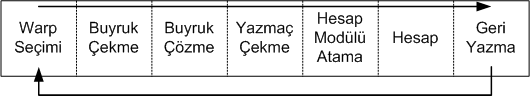
\includegraphics[width=0.9\textwidth]{gorsel/pipelineStages.png}
\shorthandoff{=}
\caption{Tosun Boru Hattı Mimarisi}
\label{image:pipelineStages}
\end{figure}

\subsection{Warp Seçimi}
Warp NVidia tarafından literatüre kazandırılmış bir terimdir. Threadlerin bir araya toplanması ile oluşan thread grubuna warp ismi verilmiştir. Thread sözlükte ipliğe karşılık gelirken warp da dokumacılıkta kullanılan çözgü anlamını taşımaktadır. N adet threade sahip bir uygulamanın M adet SIMD Lane kapasitesi bulunan bir işlemcide çalıştırılması senaryosunda 3 farklı ihtimal vardır. N = M ise her bir SIMD lane üzerinde bir thread koşturulur. N < M ise bazı SIMD lane'ler boş kalır ve bunların sonuçları değerlendirilmez. En sık rastlanan durum olan N > M olması durumunda ise N adet thread M adet kapasiteli alt gruplara bölünür ve bir seferde M adet thread çalıştırılır. Arkasından ikinci ve üçüncü M adet thread barındıran gruplar çalıştırılır. Burada her M adet thread'den oluşan gruba warp ismi verilir. Dolayısıyla warp kapasitesi donanımda tanımlı SIMD lane sayısına bağlı iken warp sayısı uygulamadaki toplam thread sayısının warp büyüklüğüne bölümü ile hesaplanır. Threadlerin warplara ayrılma işlemi derleyici tarafından yapılır.\par 
Aralıklı işlem modelinin bir uygulaması olarak, bir SIMD lane'e her saat vuruşunda farklı bir warp'a ait bir thread atanır. Hangi warp'un seçileceği boru hattının "Warp Seçimi" aşamasında belirlenir. Bu seçim Round-Robin politikasına göre gerçekleştirilir. Her warp için durum bitleri tutulur. Bu bitler warp'un "yürütme için uygun", "çalışıyor", "tamamlandı" gibi durumlarını gösterir. Uygun olan warp'lardan biri seçilir ve bu warp'un numarası boru hattının bir sonraki aşamasına aktarılır. Seçilen warp, boru hattını tamamlamadan bir daha seçilememesi için durum bitleri değiştirilerek işaretlenir. Aynı warp'un bir kez daha boru hattına alınması thread'lerin bir sonraki buyruklarının işlenmesi anlamına gelir. Bir warp boru hattını tamamlamadan ikinci kez boru hattına alınmadığında ikinci buyruk da boru hattına girmemiş olacağından herhangi bir veri bağımlılığı kontrolüne gerek kalmaz.\par
\subsection{Buyruk Çekme}
Buyruk çekme aşamasında bir önceki aşamadan gelen warp id'nin sıradaki buyruğu bellekten çekilir. Program buyrukları harici RAM’de tutulur. Buyruklara erişim program akışı sebebiyle genel olarak sıralı ve aralıklı işlem modeline göre tekrarlı olduğu için RAM’den gelen buyrukları bir süre Buyruk Önbelleği yapısında tutmak bu aşamayı oldukça hızlandıran bir optimizasyondur. Buyruğun çekilmesi ile bu aşama tamamlanır ve buyruk bir sonraki aşamaya geçirilir.
\subsection{Buyruk Çözme}
Bu aşamada buyruk çözümlenerek hangi işlem biriminin kullanılacağı, hangi yazmaçların okunup, hangilerine yazılacağı belirlenir. Tüm buyrukların 32 bit olması, işlem kodu genişliklerinin buyruklar arasında fazla farklılık göstermemesi ve neredeyse tüm buyrukların aynı yazmaçlara erişim yapabilmesinden dolayı, boru hattının bu aşaması sade bir yapıdadır.
\subsection{Yazmaç Çekme}
Burada çalıştırılmak üzere olan buyruğun işlem sırasında kullanacağı verilen yazmaç öbeğinden alınır. Her bir SIMD lane üzerinde her bir warp için ayrı bir Yazmaç Öbeği vardır ve bunlardan kullanılacak veriler aynı anda çekilir. İki adet kaynak yazmacı bulunan buyruklarda ve 16 çekirdekli bir adada toplam 32 (16 x 2) adet 32-bitlik veri ortalama 1 çevrimde okunur.
\subsection{Hesap Modülü Atama}
Boru hattının bu aşaması hesaplamanın başlatıldığı yerdir. Bu aşamaya gelen bir buyruğun tüm verileri hesaplamaya hazır bir halde beklemektedir. Bu aşamada işlem koduna bakılarak buyruk gerekli hesaplama donanımına gönderilir.
\subsection{Hesap}
Hesaplamanın yapıldığı aşamadır. Burada birçok işlem birimi yer alır. Bunlardan, sık kullanılan ve daha az alan kaplayan işlem birimleri SIMD lane adetindedir. Bu şekilde, bu işlem birimleri gelen tüm verileri aynı anda işleme sokabilecek durumdadır. Daha nadir erişilen trigonometrik işlemler ve logaritma gibi hesaplardan sorumlu işlem birimleri ise daha az sayıda bulunabilir. Az sayıda bulunan işlem birimlerinin kendi boru hattı mevcuttur. Örneğin SIMD lane sayısının yarısı adetinde olan bir hesaplama modülü ilk çevrimde gelen sayıların yarısını işleme alır, ikinci çevrimde ise diğer yarısını işleme alır. Böylece tüm sayılar boru hattında peşi sıra ilerlemiş olurlar. Örneğin 28 çevrim süren bir sinus işlemi için SIMD lane sayısının çeyreği kadar sinus hesaplama birimi yerleştirilmişse, tüm sayıların sinus sonuçlarının hesaplanması 28 + 3 = 31 çevrim sürer. Alan kullanımı ve performans optimizasyonu için esneklik sağlayan bu yapıda ilave 3 çevrim kabul edilerek alandan kazanılabilir ya da hesap modülü sayısı artırılarak performans artışı sağlanabilir. Hesap aşamasının sonunda bir sonuç buffer'ı bulunmaktadır. Hesap modüllerinin boru hattından çıkan sonuçlar önce bu buffer'lara yazılır ve yazılmak için kendi sıralarının gelmesini beklerler. 
\subsection{Geri Yazma}
Geri yazma aşaması sonuçların yazmaç öbeklerine yazıldığı aşamadır. Geri yazma aşamasının kontrolcüsü sürekli olarak hesap modüllerinin çıkışlarındaki sonuç buffer'larını kontrol eder ve sırasıyla sonuçları ilgili yazmaçlara yazar.

\section{Veri Yolu Mimarisi }
Önceki bölümlerde Tosun mimarisinin buyruk kümesi, hesaplama donanımları ve boru hattı aşamaları belirlenmiştir. Parçaların birleştirilmesi ile veri yolu mimarisi oluşacaktır. Tasarım gereksinimleri arasında belirtilen ölçkelenebilirlik özelliğinden dolayı tüm kodlama parametrik olarak yapılmıştır. Mimarinin üzerine inşa edildiği temel parametrelerden biri de SIMD lane sayısıdır. SIMD lane sayısındaki artış, veri yolu genişliklerinin, karşılaştırıcı, kod çözücü ve kodlayıcı gibi donanımların katlanarak artmasına sebep olmaktadır. Bu etki hem alan kullanımında hem de sinyal gecikmelerinde artışa neden olur. Neticede performans kaygısı ile paralelliğin artması için SIMD lane sayısının artırılması ile alan kullanımı büyümekte, gecikmeler artmakta ve hem güç tüketimi artmakta hem saat sıklığı azalmaktadır. Dahası FPGA içi routing işlemi de SIMD lane sayısının artması ile zorlaşmakta ve imkansız hale gelebilmektedir. Bu etki, kaçınılmaz olmakla beraber hiyerarşik tasarım kullanılarak azaltılabilir.\par 

Tosun mimarisi routing ve timing ile ilgili kısıtları zorlayabilmek adına hiyerarşik bir yapıda tasarlanmıştır. Doğrudan N adet SIMD lane gerçeklenmesi yerine küçük gruplar halinde, $N=N_{1}xN_{2}$ olacak şekilde $N_{1}$ adet ada ve her adanın içinde $N_{2}$ adet SIMD lane olacak şekilde gerçeklenmiştir. Hiyerarşinin üst seviyesinde, ölçeklenebilirliği olmayan PCI-e ve Ana bellek arayüzü gerçeklenmiş ve AXI bus yapısı ile N adet ada ismi verilen donanıma bağlanmıştır. Tosun üst seviye mimari çizimi Şekil \ref{image:genelMimari}’da sunulmuştur. Mimarinin büyük tek bir ada yerine çok sayıda daha küçük adalardan oluşmasının iki sebebi  vardır. \par
\begin{figure}[h]
\centering
\shorthandoff{=}
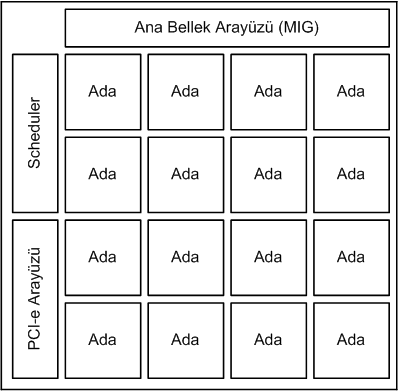
\includegraphics[width=0.5\textwidth]{gorsel/genelMimari.png}
\shorthandoff{=}
\caption{Tosun Üst Seviye Mimarisi}
\label{image:genelMimari}
\end{figure}
Her bir ada içindeki threadlerin veri paylaşabilmesi için ada içine yerleştirilen paylaşımlı belleğe erişimi olan çekirdek sayısı ile bu bellekte yaşanan gecikme doğrudan ilişkilidir. Paylaşımlı bellek açısından bakıldığında istemci sayısının artması istek paketlerinin beklediği kuyrukta uzamaya sebep olmaktadır. Bu durum sınav zamanında kütüphaneden kitap almak isteye öğrenciler analojisiyle açıklanabilir. Her bir öğrenci bir istek paketi, ulaşmak istedikleri kitaplar da paylaşımlı bellekte tutulan veriler olsun. Kütüphanede kitap ödünç alımıyla ilgilenen personel sayısını sabit olarak 2 kabul edelim. Kitap sayısı sonsuz bile olsa, N adet öğrencinin bu iki personel üzerinden kitaplara erişim imkanı varken, öğrenci sayısının artması ile bir öğrencinin ortalama kitaba ulaşma süresi doğru orantılı olarak artacaktır. Artışı engellemek için yapılabilecek iki seçenekten birincisi öğrenci sayısını sınırlamak, ikincisi ise personel sayısını artırmaktır. Bu analojide personel sayısı FPGA üzerinde gerçeklenen Block RAM'lerin port sayısını ifade eder. Block RAM'lerin port sayısı 2'den fazla olamadığından istemci sayısını azaltmak tek çözümdür. Bu bağlamda tasarımı adalara ayırmak, kütüphaneyi parçalamaya ve kütüphane başına düşen öğrenci sayısını azaltmaya benzer. Dolayısıyla çok sayıda çekirdeği küçük gruplar halinde ayırarak her gruba bir paylaşımlı bellek tahsis etmek bellek işlemlerinin performansını artıracaktır. \par
Diğer bir sebep ise yukarıda bahsedilen, FPGA gerçeklemesi sırasında oluşabilecek timing ve routing problemleridir. Yapılan bir tasarım FPGA üzerinde gerçeklenirken herhangi bir kısıt tanımlanmamışsa birbirine yakın olması beklenen bazı donanım parçaları yonga üzerinde uzak yerlere denk gelebilir. Ölçeklenebilir tasarımlarda bu problem sıklıkla kaynakların verimsiz kullanımına ve tellerin uzaması ile kritik yollardaki gecikmelerin artmasına dolayısıyla saat frekansının düşmesine ve nihayetinde performans düşüşüne sebep olabilir. Bu problemlerden kaçınmak için sıklıkla hiyerarşik tasarımlar gündemde tutulur. Tosun tasarımının homojen adalardan oluşması sentez aracına hangi donanımların yakın olması gerektiği konusunda daha çok fikir vermekte ve bu konudaki potansiyel problemlerin indirgenmesine olanak sağlamaktadır.\par 
Tasarımın adalara ayrılması ile donanım seviyesinde bir soyutlama sağlanmıştır. Bu soyutlama, Tosun üzerinde o anda koşan tüm threadlerin aynı anda aynı buyruklarının koşması zorunluluğunu ortadan kaldırır. SIMD mimarinin bir özelliği olarak herhangi bir t anında ada içerisinde çalışan tüm threadlerin aynı buyrukları koşmakta, bütün threadler için o buyruk tamamlanmadan diğer buyruğa geçilmemektedir. Öte yandan aynı anda farklı adalarda farklı buyruklar çalışıyor olabilir. Bu sayede ana bellek erişimi farklı adalar için farklı zamanlarda gerçekleşebilir; böyle bir durumda beklemeler azalır. Farklı adaların farklı zamanlarda bellek erişimi istemesi ise ilk bellek erişiminden sonra kaçınılmazdır.  

\subsection{Ada İçi Veri Yolu Mimarisi}

Yukarıda anlatılan buyrukların koşturulduğu ve boru hattının uygulandığı mimari ada içi mimaridir. Her adanın içinde N adet SIMD lane var ise N adet yazmaç öbeği bulunmaktadır. Alan tüketimi az olan ve hedef uygulamalarda sıkça kullanılan hesaplama birimlerinden de N adet bulunmaktadır. Diğer buyruklara oranla daha az sıklıkta kullanılan ve alan tüketimi yüksek olan hesaplama birimlerinden ise $N/2^{k}, k\in Z^{+} , 1 \le k \le log_{2}N$ adet kullanılır. Uzun süren hesaplama modüllerinin içinde de boru hattı bulunmaktadır. Bu sayede modül sayısının $N/2^{k}$ olduğu durumda sadece k çevrim maliyeti olur.\par
\begin{figure}[h]
\centering
\shorthandoff{=}
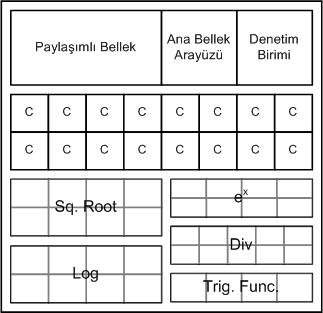
\includegraphics[width=0.5\textwidth]{gorsel/adaMimarisiEski.png}
\shorthandoff{=}
\caption{Tosun Ada Mimarisi (Kavramsal)}
\label{image:adaMimarisiEski}
\end{figure}

\begin{figure}[h]
\centering
\shorthandoff{=}
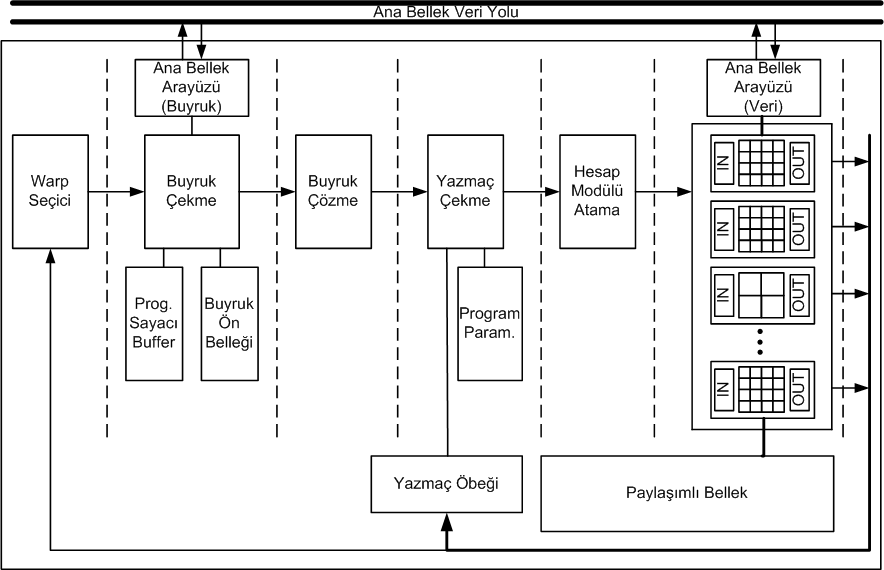
\includegraphics[width=0.9\textwidth]{gorsel/adaMimarisi.png}
\shorthandoff{=}
\caption{Tosun Ada Mimarisi (Boru Hattı)}
\label{image:adaMimarisi}
\end{figure}

Ada içi mimarinin kavramsal gösterimi şekil \ref{image:adaMimarisiEski}'de boru hattı ile gösterimi şekil \ref{image:adaMimarisi}'de sunulmuştur. Her bir buyruk boru hattı üzerinde ilerleyerek işlenir. Boru hattının etkin kullanımı için daha önce belirtilen aralıklı işlem modeli kullanılır ve her saat vuruşunda farklı bir warptan işlem alınır. \par
Bir adada koşturulan thread sayısı adanın SIMD lane sayısı kadardır. Aralıklı işlem modelinin uygulanabilmesi için adada koşturulan warplara ait yazmaç bilgilerinin tamamının yazmaç öbeğinde saklanması gerekir. Dolayısıyla adada koşturulan warp sayısı yazmaç öbeğinin büyüklüğüne bağlıdır.\par

\subsubsection{Yazmaç Öbeği Tasarımı}
NVidia benchmarkları üzerinde yapılan analizlerde thread başına 64 yazmacın yeterli olacağı tespit edilmiş ve buyruk kümesi de 64 yazmaca göre tasarlanmıştır. Aralıklı işlem modelinin uygulanabilmesi için her saat vuruşunda yeni bir warp'un boru hattına alınması gerekmektedir. Ana boru hattı 7 aşamadan oluşmakta, hesaplama işlemleri ise 28 vuruşa kadar çıkmaktadır. Boru hattını doldurabilecek sayıda olması açısından ada içindeki warp sayısının minimum 32 olması gerekmektedir. Dolayısıyla her bir SIMD lane için yazmaç öbeği büyüklüğü 64 yazmaç x 32 warp x 32bit = 64kbit kapasiteli olmalıdır. 32kbit büyüklüğünde 2 block ram primitive kullanılarak yazmaç öbeği tasarlanabilir.\par
\begin{figure}[h]
\centering
\shorthandoff{=}
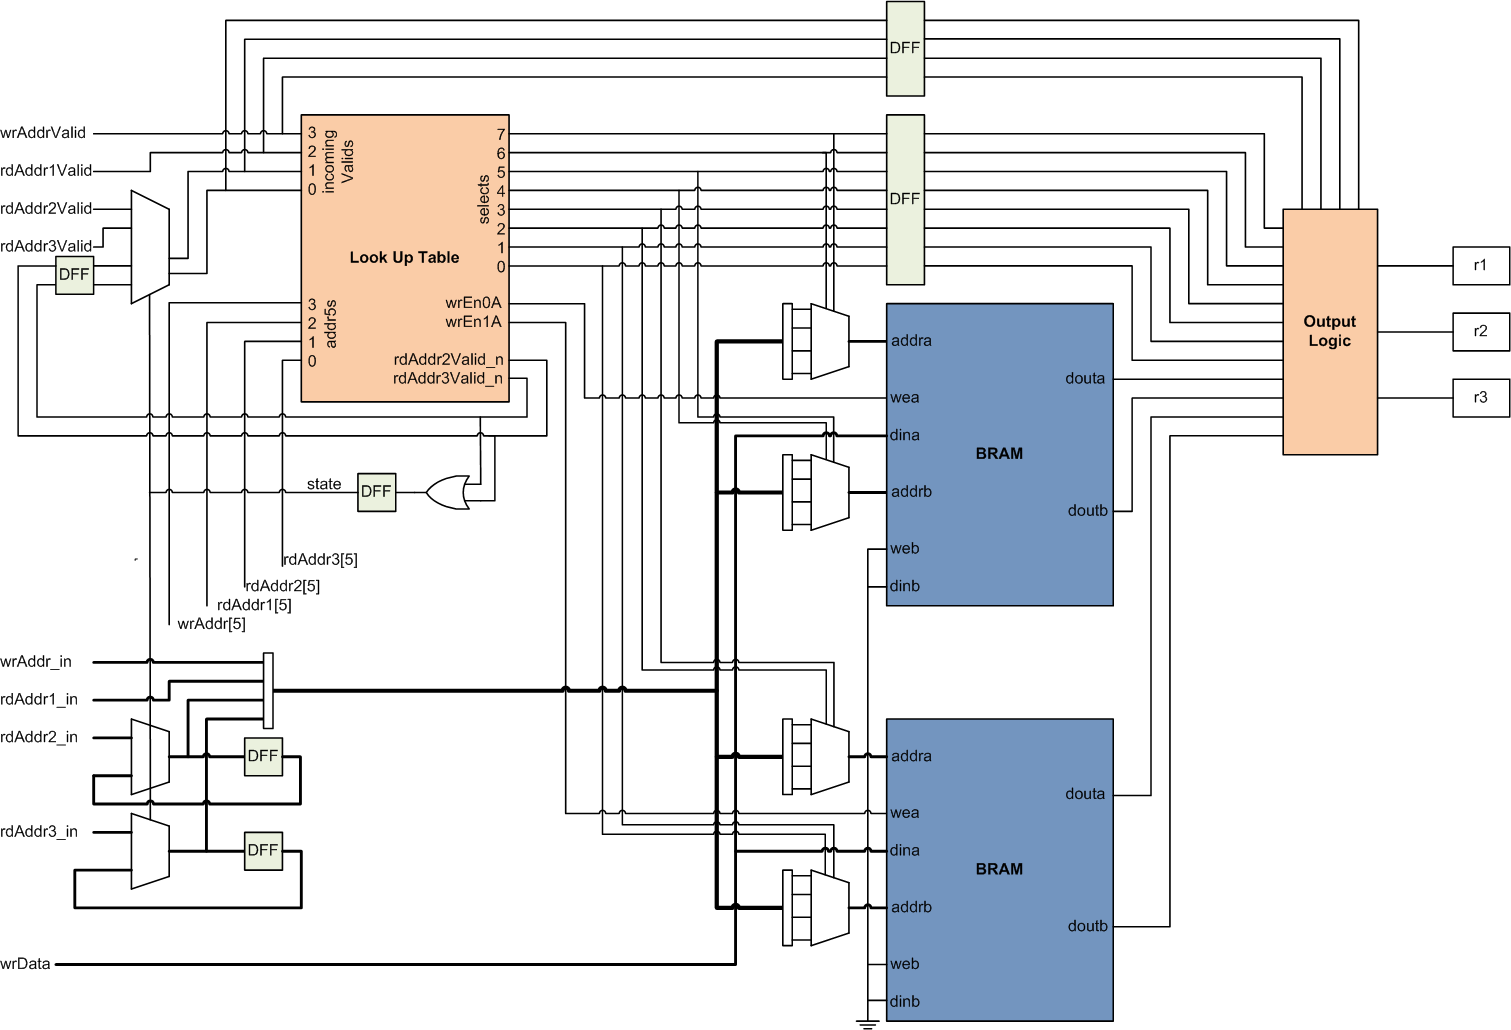
\includegraphics[width=\textwidth]{gorsel/registerFile.png}
\shorthandoff{=}
\caption{Tosun Yazmaç Öbeği}
\label{image:registerFile}
\end{figure}
Şekil \ref{image:registerFile}’de gösterilen yazmaç öbeği 2 adet true dual port BRAM kullanmaktadır. Dolayısıyla toplam 4 adet fiziksel port bulunur. Buyruk kümesinde var olan buyruklara göre aynı anda en fazla 3 okuma ve 1 yazma operasyonu (4 portlu) gelmektedir. 4 port üzerinden gelen isteklerin BRAM’lere bağlı 4 porta aktarılabilmesi için adreslerin 2’şerli gruplandığında farklı BRAM’leri göstermesi gerekir. Bu durumun her zaman olacağı garanti edilemeyeceğinden portlara bir öncelik ataması yapılmış (WR > RD1 > RD2 > RD3) ve önceliği düşük olan 2 portun sonraki çevrim(ler)de işlenebilmesi için gerekli hafıza birimleri yerleştirilmiştir. Burada en kötü durum tüm portların aynı BRAM’e ait adresleri göstermesidir.  Böyle bir durum oluştuğunda WR ve RD1 portunun istekleri aynı çevrimde işlenirken RD2 ve RD3 portları sonraki çevrimde işlenmek üzere bekletilir. Eğer sonraki çevrimde yeni bir WR operasyonu gelirse WR ve RD2 işlenir, RD3 bekletilir. Nihayetinde en kötü durumda 3. Çevrimde RD3’ün de okunması ile okuma işlemi tamamlanmış olur. Özetle Şekil \ref{image:registerFile}’de gösterilen tasarıma sahip bir yazmaç öbeği kümesinde bulunan yazmaç öbeklerinde en kötü durum için yazma işlemi 1 çevrimde okuma işlemi 3 çevrimde tamamlanmaktadır. Bu gecikmeler BRAM kısıtlarından kaynaklanmaktadır. \par
Yazmaç öbeği okuma işlemlerinin en kötü durumdaki cevap süresini kısaltmak mümkün olmasa da en kötü durumun oluşma ihtimalini azaltmak mümkündür. Bir iyileştirme olarak her bir thread’e ait 64 adet yazmaçtan oluşan yazmaç öbeği, 32 yazmaçlık 2’şer gruba bölünerek tüm thread’lere ait yazmaç öbeklerinin ilk yarıları ilk BRAM’de, ikinci yarıları ise ikinci BRAM’de saklanır. Bu saklama şekli sabit tutularak derleyicinin yazmaçları seçerken bu ayrımı göz önünde bulundurulması sağlanmakta ve en kötü durumun oluşma ihtimali en aza indirgenmektedir. \par
Yazmaç Öbeği Kümesi 11 bit ile adreslenir. Soldaki 5 bit warp numarasını, sağdaki 6 bit ise yazmaç numarasını belirtir. Bu şekilde farklı bir warp'a geçiş yapılacağı zaman sadece bu adresin 5 bitlik prefix’inin değiştirilmesi yeterli olur. Dolayısıyla hiç saat vuruşu kaybetmeden context switch yapılabilir.
\subsubsection{Hesaplama Modülleri}
Tüm işlemler için hesaplama modüllerinin yapısı aynıdır. Giriş ve çıkışlardan da sadece “sayılar” girişleri içerideki birime göre değişken olabilir, diğer tüm giriş ve çıkışlar ise standarttır. Örneğin; toplama birimi için 2 adet 32-bitlik giriş varken, multiply-add işlemi için 3 adet sayı gerekir. Şekil \ref{image:executionUnitIO}'de “N” hesaplamada kullanılan eleman sayısını göstermektedir.\par
\begin{figure}
\centering
\shorthandoff{=}
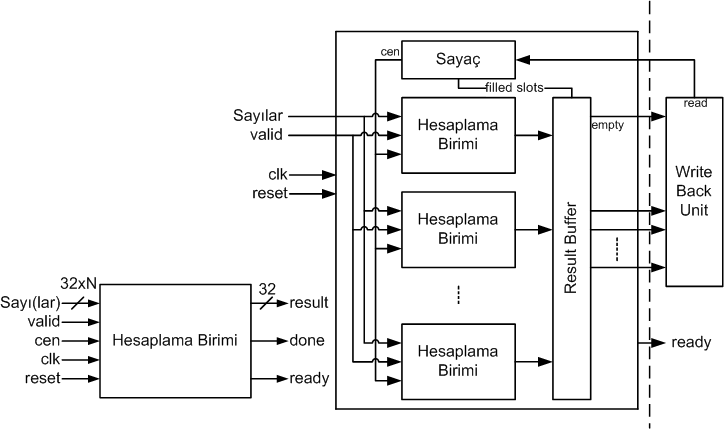
\includegraphics[width=0.9\textwidth]{gorsel/executionUnitIO.png}
\shorthandoff{=}
\caption{Hesaplama Modülleri}
\label{image:executionUnitIO}
\end{figure}
Hesaplama modülleri \ref{image:executionUnitIO}'de sağ tarafta gösterildiği gibi Hesaplama Grubu’nu oluşturur. Burada en fazla çekirdek sayısı kadar olmak üzere değişken sayıda işlem birimi yer alabilir. Grup içerisindeki işlem birimlerinin paylaştığı  Sonuç Buffer'ı vardır. Sonuç Buffer'ı yine Hesaplama Grubu içerisinde yer alan “sayaç” ile birlikte bir FIFO yapısı gibi davranır. Hesaplama Birimlerinden çıkan sonuçlar Sonuç Buffer’ına yazılır ve "Geri-Yazma" biriminin bu verileri okuyup yazmaç öbeğine yazması beklenir. Geri yazma birimi round robin algoritmasını kullanarak hazır olan verileri sıradan yazmaç öbeğine yazar.

\subsubsection{Paylaşımlı Bellek}
Threadlerin yazmaçları kendilerine özel olup dışarıdan bir modülün erişimi yoktur. Oysa ki paralel hesaplamalarda bir threadin ürettiği bir sonuç başka bir thread tarafından kullanılabilir. Threadler arası veri paylaşımı için iki seçenek vardır. Bir seçenek ana bellek üzerinden veri paylaşımı yapılması iken diğeri paylaşımlı bellek eklenmesidir. Ana bellek hem yonga dışında olduğundan hem de veri yolu genişliğinin sınırlı olmasından dolayı yavaş olacaktır.\par
FPGA üstünde paylaşımlı bellek gerçeklemesi ancak Block RAM kullanımı ile mümkündür. Donanımda tanımlı Block RAM Primitive'ler 32kbit büyüklüğünde olup 2 portu desteklemektedir. Paylaşımlı bellek kapasitesinin artırılması birden fazla Block RAM Primitive üzerine adres uzayı taksim edilir.\par
Her bir çekirdeğin paylaşımlı belleğe erişiminin bulunması gerekmektedir. Bunun için çekirdek sayısı adetinde porta sahip bir paylaşımlı bellek Block RAM Primitive'ler kullanılarak Şekil \ref{image:sharedMemory}'de gösterildiği şekilde tasarlanmıştır.
\begin{figure}[ht]
\centering
\shorthandoff{=}
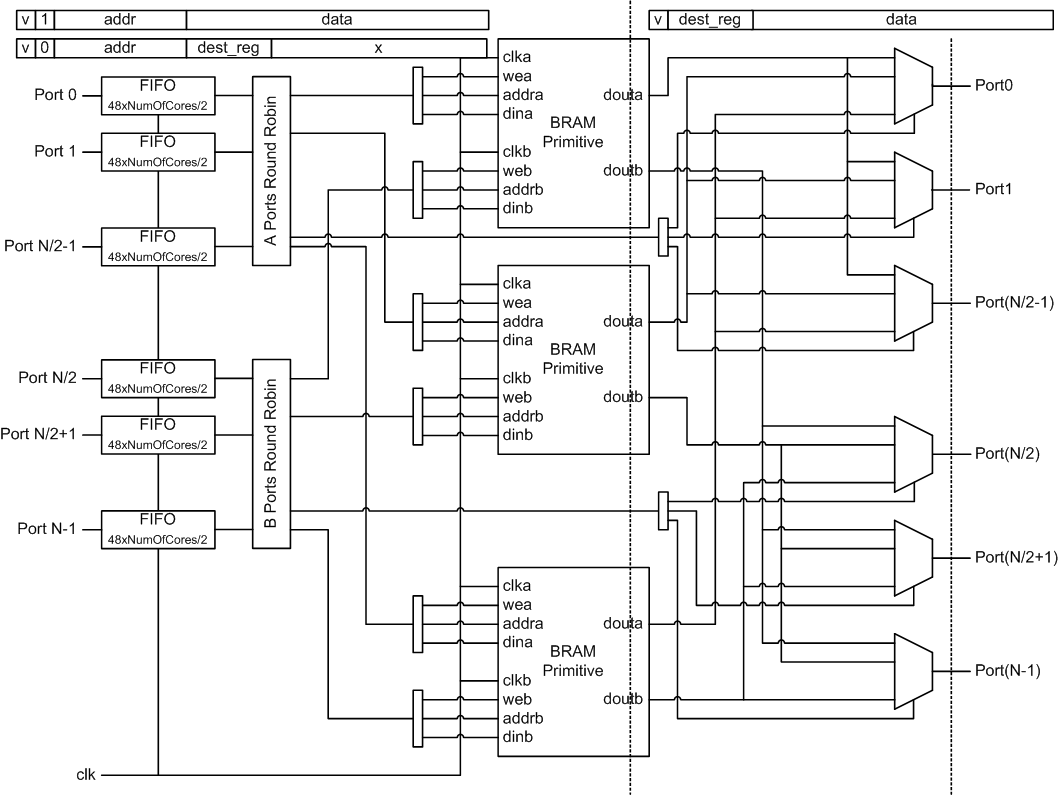
\includegraphics[width=0.9\textwidth]{gorsel/sharedMemory.png}
\shorthandoff{=}
\caption{Tosun Paylaşımlı Belllek Mimarisi}
\label{image:sharedMemory}
\end{figure}

Paylaşımlı belleğin girişindeki her bir port bir SIMD lane'e bağlıdır. Paylaşımlı belleğin içinde N adet 32kbit Block RAM Primitive şekil \ref{image:sharedMemory}'de gösterildiği gibi giriş portlarına öncelik atayıcı donanımlar üzerinden bağlıdır. Her block ram portu için bir öncelik atayıcı bulunmakta ve o block ram portunun hangi SIMD lane portu ile bağlanacağına karar vermektedir. Herhangi SIMD lane üzerinde paylaşımlı belleğe yazma veya okuma amaçlı erişmek isteyen bir buyruk olursa, o SIMD lane'e bağlı port üzerinden ilgili öncelik atayıcıya istek gelir. Her saat vuruşunda öncelik atayıcılar kendilerine gelen istekler üzerinden Round Robin algoritması ile bir seçim yapar. Seçilen paket block ram'e iletilirken, seçilmeyen paketler sırada tutulur. Bunun için her SIMD lane portunun girişinde bir FIFO tampon bellek bulunmaktadır. Her block ram primitive 2 adet porta sahip olduğu için SIMD lane portları ikiye bölünür. Yarısı block ram primitive'lerin A portlarına bağlanırken diğer yarısı B portlarına bağlanır.\par

Paylaşımlı bellek mimarisi için en kötü durum tüm SIMD lane portlarından aynı block RAM primitive için istek paketleri gelmesidir. Bu durumda SIMD lane sayısının yarısı büyüklüğünde kuyruk oluşur ve işlemler buna göre gecikmeli gerçekleşir. En kötü durum ihtimalini ortadan kaldırmak mümkün değildir fakat ihtimali düşürmek adına adres uzayının block ram'lere dağıtım yönteminde iyileştirme yapılabilir. \par

Tosun paylaşımlı bellek mimarisinde kullanılan verilerin tamamı 32 bit genişliğinde, block ram primitiveler ise 32 kbit büyüklüğündedir. Dolayısıyla her block ram primitive 1000 adet adresten oluşur. Paylaşımlı bellek büyüklüğünün 128kbit olması durumunda toplamda 8 adet block ram bulunmaktadır Adres uzayı block ramlere paylaştırılırken üst bitler yerine alt bitlerin kullanılması ile ardışık adresler her zaman farklı block ram primitive'lerini gösterir ve en kötü durum ihtimali azaltılır. 

\chapter{SONUÇ}

\newpage
\pagestyle{plain}
\addcontentsline{toc}{chapter}{\numberline{KAYNAKLAR}}


\begin{thebibliography}{99}

\bibitem{cudaProgrammingStructure} Lippert, A. (2009). NVIDIA GPU Architecture for General Purpose Computing, 18.

\bibitem{dspArchitectures} Edwin. J. Tan, Wendi. B. Heinzelman. 2003. DSP Architectures: Past, Present and Futures. ACM Sigarch Computer Architecture News

\bibitem{hallmans2013gpgpu} Hallmans, Daniel, et al. 2013. GPGPU for industrial control systems. IEEE 18th Conference on Emerging Technologies \& Factory Automation ETFA

\bibitem{Kilgariff2005} Emmett Kilgariff and Randima Fernando. 2005. The GeForce 6 series GPU architecture. In ACM SIGGRAPH 2005 Courses SIGGRAPH '05, John Fujii (Ed.). ACM, New York, NY, USA

\bibitem{kirk2007nvidia} Kirk, D. 2007. NVIDIA CUDA software and GPU parallel computing architecture. ISMM Vol. 7, pp. 103-104

\bibitem{stone2010opencl} Stone, J. E., Gohara, D., \& Shi, G. 2010. OpenCL: A parallel programming standard for heterogeneous computing systems. Computing in science \& engineering, 12(3), 66

\bibitem{kuon2007measuring} Kuon, I., \& Rose, J. 2007. Measuring the gap between FPGAs and ASICs. Computer-Aided Design of Integrated Circuits and Systems, IEEE Transactions on, 26(2), 203-215.

\bibitem{smith1997matlab}Smith, R.L., \"The MATLAB project book for linear algebra\", 1997 Prentice Hall

\bibitem{cooleyTukey} Cooley, J. W., \& Tukey, J. W. (1965). An algorithm for the machine calculation of complex Fourier series. Mathematics of computation, 19(90), 297-301.

\bibitem{eigenvalueComputation} Gotze, J.; Paul, S.; Sauer, M., \"An efficient Jacobi-like algorithm for parallel eigenvalue computation,\" Computers, IEEE Transactions on , vol.42, no.9, pp.1058,1065, Sep 1993

\bibitem{flynnTaxonomy}Flynn, M. J. (September 1972). \"Some Computer Organizations and Their Effectiveness\". IEEE Trans. Comput. C–21 (9): 948–960. doi:10.1109/TC.1972.5009071

\bibitem{shivakumar2002modeling} Shivakumar, P., Kistler, M., Keckler, S. W., Burger, D., \& Alvisi, L. (2002). Modeling the effect of technology trends on the soft error rate of combinational logic. In Dependable Systems and Networks, 2002. DSN 2002. Proceedings. International Conference on (pp. 389-398). IEEE.

\bibitem{seiler2008larrabee} Seiler, L., Carmean, D., Sprangle, E., Forsyth, T., Abrash, M., Dubey, P., ... \& Hanrahan, P. (2008). Larrabee: a many-core x86 architecture for visual computing. ACM Transactions on Graphics (TOG), 27(3), 18.

\bibitem{molka2009memory} Molka, D., Hackenberg, D., Schone, R., \& Muller, M. S. (2009, September). Memory performance and cache coherency effects on an Intel Nehalem multiprocessor system. In Parallel Architectures and Compilation Techniques, 2009. PACT'09. 18th International Conference on (pp. 261-270). IEEE

\bibitem{hackenberg2009comparing} Hackenberg, D., Molka, D., \& Nagel, W. E. (2009, December). Comparing cache architectures and coherency protocols on x86-64 multicore SMP systems. InProceedings of the 42Nd Annual IEEE/ACM International Symposium on microarchitecture (pp. 413-422). ACM

\bibitem{MCSE.2012.23} Heinecke, A., Klemm, M., Bungartz H.J., \"From GPGPU to Many-Core: Nvidia Fermi and Intel Many Integrated Core Architecture\" Computing in Science and Engineering, vol. 14, no. 2, pp. 78-83, March-April, 2012 

\bibitem{cpuGpuMemoryTable} http://supercomputingblog.com/cuda/cuda-memory-and-cache-architecture/

\bibitem{tileArchitecture} Wentzlaff, D., Griffin, P., Hoffmann, H., Bao, L., Edwards, B., Ramey, C., Mattina, M., Miao, C.-C., III, J. F. B. \& Agarwal, A. (2007). On-Chip Interconnection Architecture of the Tile Processor.. IEEE Micro, 27, 15-31. 

\bibitem{nvidiaPTXISA} http://docs.nvidia.com/cuda/parallel-thread-execution/\#texture-instructions

\bibitem{x86ISA} http://en.wikipedia.org/wiki/X86\_instruction\_listings

\bibitem{MIPSISA} http://www.mrc.uidaho.edu/mrc/people/jff/digital/MIPSir.html

\bibitem{superscalar600mhz} Gieseke, B. A., Allmon, R. L., Bailey, D. W., Benschneider, B. J., Britton, S. M., Clouser, J. D., ... \& Wilcox, K. E. (1997, February). A 600 MHz superscalar RISC microprocessor with out-of-order execution. In Solid-State Circuits Conference, 1997. Digest of Technical Papers. 43rd ISSCC., 1997 IEEE International (pp. 176-177). IEEE.

\bibitem{superscalarpatent}Garg, S., Hagiwara, Y., Lau, T. L., Lentz, D. J., Miyayama, Y., Trang, Q. H., ... \& Wang, J. (1996). U.S. Patent No. 5,560,032. Washington, DC: U.S. Patent and Trademark Office.

\bibitem{interleavedMultithreading} Laudon, J., Gupta, A., \& Horowitz, M. (1994). Interleaving: A multithreading technique targeting multiprocessors and workstations. ACM SIGPLAN Notices, 29(11), 308-318.

\bibitem{Controldatacorp}Control Data Corp, «CDC Cyber 170 Computer Systems; Models 720, 730, 750, and 760; Model 176 (Level B); CPU Instruction Set; PPU Instruction Set,» pp. 2-44.

\bibitem{TeraMTA}A. e. a. Snavely, \"Multi-processor Performance on the Tera MTA,\" in IEEE Computer Society Proceedings of the 1998 ACM/IEEE conference on Supercomputing, 1998. 


\end{thebibliography} % Kaynakca .bib seklinde degil de kaynakca.tex dosyasi olarak hazirlanirsa bu satir kullanilmali
%\bibliography{kaynakca} % kaynakca.bib dosyasi hazirlanirsa bu satir kullanilmali
%\bibliographystyle{abbrv} % kaynakca.bib ile beraber kullanim icin.
%\renewcommand{\appendixname}{}
\renewcommand{\appendixtocname}{EKLER}
\renewcommand{\appendixpagename}{EKLER}

\begin{appendices}
\appendix
\chapter{Veriler}



\chapter{Algoritma}
\end{appendices}
\newpage
\pagestyle{plain}
\addcontentsline{toc}{chapter}{\numberline{\"OZGE\c{C}M\.{I}\c{S}}}
\begin{center}
{\LARGE \bf \"OZGE\c{C}M\.{I}\c{S}}
\end{center}
\vspace{0.5cm}
{\bf Ki\c{s}isel Bilgiler}


\noindent
\begin{tabular}{@{}lll@{}}
Soyad{\i}, Ad{\i} & : Yağlıkçı, Abdullah Giray &\\
Uyru\u{g}u & : T.C.&\\
Do\u{g}um tarihi ve yeri & : 09.08.1988 Ankara&\\
Medeni hali & : Bekar& \\
Telefon & : &\\
Faks & : &\\
e-mail & : agyaglikci@.etu.edu.tr &\\
\end{tabular}

\vspace{0.5cm}
\noindent
{\bf E\u{g}itim}


\noindent
\begin{tabular}{@{}llc@{}}
{\bf Derece} & {\bf E\u{g}itim Birimi} & {\bf Mezuniyet Tarihi}\\
Y. Lisans & TOBB Ekonomi ve Teknoloji \"Universitesi & 2014\\
Lisans & TOBB Ekonomi ve Teknoloji \"Universitsi& 2011\\
\end{tabular}

\vspace{0.5cm}
\noindent
{\bf \.{I}\c{s} Deneyimi}


\noindent
\begin{tabular}{@{}lll@{}}
{\bf Y{\i}l} & {\bf Yer} & {\bf G\"orev}\\
2012-2014 & TOBB Ekonomi ve Teknoloji \"Universitesi & Burslu Yüksek Lisans Öğrencisi\\
\end{tabular}

\vspace{0.5cm}
\noindent
{\bf Yabanc{\i} Dil}


\noindent
\begin{tabular}{@{}l@{}}
\.{I}ngilizce (İleri Seviye)\\
\end{tabular}


\vspace{0.5cm}
\noindent
{\bf Yay{\i}nlar} \\
\noindent
Mustafa Cavus, Hakki Doganer Sumerkan, Osman Seckin Simsek, Hasan Hassan, Abdullah Giray Yaglikci, Oguz Ergin: GPU based Parallel Image Processing Library for Embedded Systems. VISAPP 2014




\end{document}
